%%%%%%%%%%%%%%%%%%%%%%%%%%%%%%%%%%%%%%%%%
% Masters/Doctoral Thesis 
% LaTeX Template
% Version 2.5 (27/8/17)
%
% This template was downloaded from:
% http://www.LaTeXTemplates.com
%
% Version 2.x major modifications by:
% Vel (vel@latextemplates.com)
%
% This template is based on a template by:
% Steve Gunn (http://users.ecs.soton.ac.uk/srg/softwaretools/document/templates/)
% Sunil Patel (http://www.sunilpatel.co.uk/thesis-template/)
%
% Template license:
% CC BY-NC-SA 3.0 (http://creativecommons.org/licenses/by-nc-sa/3.0/)
%
%%%%%%%%%%%%%%%%%%%%%%%%%%%%%%%%%%%%%%%%%

%----------------------------------------------------------------------------------------
%	PACKAGES AND OTHER DOCUMENT CONFIGURATIONS
%----------------------------------------------------------------------------------------

\documentclass[
11pt, % The default document font size, options: 10pt, 11pt, 12pt
%oneside, % Two side (alternating margins) for binding by default, uncomment to switch to one side
english, % ngerman for German
doublespacing, % Single line spacing, alternatives: singlespacing, onehalfspacing or doublespacing
%draft, % Uncomment to enable draft mode (no pictures, no links, overfull hboxes indicated)
%nolistspacing, % If the document is onehalfspacing or doublespacing, uncomment this to set spacing in lists to single
%liststotoc, % Uncomment to add the list of figures/tables/etc to the table of contents
%toctotoc, % Uncomment to add the main table of cocdntents to the table of contents
%parskip, % Uncomment to add space between paragraphs
%nohyperref, % Uncomment to not load the hyperref package
headsepline, % Uncomment to get a line under the header
%chapterinoneline, % Uncomment to place the chapter title next to the number on one line
%consistentlayout, % Uncomment to change the layout of the declaration, abstract and acknowledgements pages to match the default layout
]{MastersDoctoralThesis} % The class file specifying the document structure

\usepackage[utf8]{inputenc} % Required for inputting international characters
\usepackage[T1]{fontenc} % Output font encoding for international characters

\usepackage{mathpazo} % Use the Palatino font by default

\usepackage[backend=bibtex,style=authoryear,natbib=true,maxcitenames=2]{biblatex} % Use the bibtex backend with the authoryear citation style (which resembles APA)

%----------------------------------------------------------------------------------------

\addbibresource{thesis.bib} % The filename of the bibliography 

%----------------------------------------------------------------------------------------

\newcommand{\wmk}{Wm$^{-1}$K$^{-1}$}
\newcommand{\wmks}{Wm$^{-1}$K$^{-1}$ }

\newcommand{\Tc}{Thermal conductivity }
\newcommand{\tcs}{thermal conductivity }
\newcommand{\tc}{thermal conductivity}

\newcommand{\Co}{Conductivity }
\newcommand{\cs}{conductivity }
\newcommand{\co}{conductivity}

\newcommand{\mgsio}{MgSiO$_3$}
\newcommand{\mgsios}{MgSiO$_3$ }
\newcommand{\fesio}{FeSiO$_3$}
\newcommand{\fesios}{FeSiO$_3$ }
\newcommand{\mgfesio}{(Mg,Fe)SiO$_3$}
\newcommand{\mgfesios}{(Mg,Fe)SiO$_3$ }

%----------------------------------------------------------------------------------------

\usepackage[autostyle=true]{csquotes} % Required to generate language-dependent quotes in the bibliography

%----------------------------------------------------------------------------------------
%	MARGIN SETTINGS
%----------------------------------------------------------------------------------------

\geometry{
	paper=a4paper, % Change to letterpaper for US letter
	inner=2.5cm, % Inner margin
	outer=3.8cm, % Outer margin
	bindingoffset=.5cm, % Binding offset
	top=1.5cm, % Top margin
	bottom=1.5cm, % Bottom margin
	%showframe, % Uncomment to show how the type block is set on the page
}

%----------------------------------------------------------------------------------------
%	THESIS INFORMATION
%----------------------------------------------------------------------------------------

\thesistitle{Simulating the thermal conductivity of lower mantle minerals} % Your thesis title, this is used in the title and abstract, print it elsewhere with \ttitle

\supervisor{Dr. Stephen \textsc{Stackhouse} \\ Dr. Andrew M. \textsc{Walker} \\ Dr. Jon E. \textsc{Mound}} % Your supervisor's name, this is used in the title page, print it elsewhere with \supname

%\supervisor{Dr. Stephen \textsc{Stackhouse}}

\examiner{} % Your examiner's name, this is not currently used anywhere in the template, print it elsewhere with \examname
\degree{Doctor of Philosophy} % Your degree name, this is used in the title page and abstract, print it elsewhere with \degreename
\author{Ben \textsc{Todd}} % Your name, this is used in the title page and abstract, print it elsewhere with \authorname
\addresses{} % Your address, this is not currently used anywhere in the template, print it elsewhere with \addressname

\subject{Geophysical Science} % Your subject area, this is not currently used anywhere in the template, print it elsewhere with \subjectname
\keywords{} % Keywords for your thesis, this is not currently used anywhere in the template, print it elsewhere with \keywordnames
\university{\href{https://www.leeds.ac.uk/}{University of Leeds}} % Your university's name and URL, this is used in the title page and abstract, print it elsewhere with \univname
\department{\href{https://www.see.leeds.ac.uk}{School of Earth and Environment}} % Your department's name and URL, this is used in the title page and abstract, print it elsewhere with \deptname
\group{\href{https://www.see.leeds.ac.uk/research/igt/}{Institute of Geophysics and Tectonics}} % Your research group's name and URL, this is used in the title page, print it elsewhere with \groupname


\faculty{\href{https://www.environment.leeds.ac.uk/}{Faculty of Environment}} % Your faculty's name and URL, this is used in the title page and abstract, print it elsewhere with \facname

\AtBeginDocument{
\hypersetup{pdftitle=\ttitle} % Set the PDF's title to your title
\hypersetup{pdfauthor=\authorname} % Set the PDF's author to your name
\hypersetup{pdfkeywords=\keywordnames} % Set the PDF's keywords to your keywords
}

\begin{document}

\frontmatter % Use roman page numbering style (i, ii, iii, iv...) for the pre-content pages

\pagestyle{plain} % Default to the plain heading style until the thesis style is called for the body content

%----------------------------------------------------------------------------------------
%	TITLE PAGE
%----------------------------------------------------------------------------------------

\begin{titlepage}
\begin{center}

\vspace*{.06\textheight}
{\scshape\LARGE \univname\par}\vspace{1.5cm} % University name
\textsc{\Large Doctoral Thesis}\\[0.5cm] % Thesis type

\HRule \\[0.4cm] % Horizontal line
{\huge \bfseries \ttitle\par}\vspace{0.4cm} % Thesis title
\HRule \\[1.5cm] % Horizontal line
 
\begin{minipage}[t]{0.4\textwidth}
\begin{flushleft} \large
\emph{Author:}\\
\href{https://www.see.leeds.ac.uk/people/b.todd}{\authorname} % Author name - remove the \href bracket to remove the link 
\end{flushleft}
\end{minipage}
\begin{minipage}[t]{0.4\textwidth}
\begin{flushright} \large
\emph{Supervisor:} \\
\supname % Supervisor name - remove the \href bracket to remove the link  

% \href{http://www.jamessmith.com}{\supname} 

\end{flushright}
\end{minipage}\\[3cm]
 
\vfill

\large \textit{A thesis submitted in fulfillment of the requirements\\ for the degree of \degreename}\\[0.3cm] % University requirement text
\textit{in the}\\[0.4cm]
\groupname\\\deptname\\[2cm] % Research group name and department name
 
\vfill

{\large \today}\\[4cm] % Date
%
\includegraphics{UoL_shield} % University/department logo - uncomment to place it
 
\vfill
\end{center}
\end{titlepage}

%----------------------------------------------------------------------------------------
%	DECLARATION PAGE
%----------------------------------------------------------------------------------------

\begin{declaration}
\addchaptertocentry{\authorshipname} % Add the declaration to the table of contents
\noindent I, \authorname, declare that this thesis titled, \enquote{\ttitle} and the work presented in it are my own. I confirm that:

\begin{itemize} 
\item This work was done wholly or mainly while in candidature for a research degree at this University.
\item Where any part of this thesis has previously been submitted for a degree or any other qualification at this University or any other institution, this has been clearly stated.
\item Where I have consulted the published work of others, this is always clearly attributed.
\item Where I have quoted from the work of others, the source is always given. With the exception of such quotations, this thesis is entirely my own work.
\item I have acknowledged all main sources of help.
\item Where the thesis is based on work done by myself jointly with others, I have made clear exactly what was done by others and what I have contributed myself.\\
\end{itemize}
 
\noindent Signed:\\
\rule[0.5em]{25em}{0.5pt} % This prints a line for the signature
 
\noindent Date:\\
\rule[0.5em]{25em}{0.5pt} % This prints a line to write the date
\end{declaration}

\cleardoublepage

%----------------------------------------------------------------------------------------
%	QUOTATION PAGE
%----------------------------------------------------------------------------------------

\vspace*{0.05\textheight} %\vspace*{0.02\textheight}

{\itshape \begin{center} 
Do it! \\Just do it!
\linebreak \\
Don't let your dreams be dreams.\\Yesterday you said tomorrow, so just do it!\\Make your dreams come true!\\Just do it!
\linebreak \\
Some people dream of success,\\while you're gonna wake up,\\ and work hard at it!\\Nothing is impossible!
\linebreak \\ 
You should get to the point,\\where anyone else would quit,\\and you're not going to stop there.\\No, what are you waiting for?
\linebreak \\
Do it!\\Just do it!\\Yes you can!\\Just do it!
\linebreak \\
If you're tired of starting over,\\stop giving up.
\end{center}}\bigbreak

\hfill Shia LeBeouf %https://genius.com/Shia-labeouf-just-do-it-motivational-speech-annotated

%\noindent\enquote{\itshape Thanks to my solid academic training, today I can write hundreds of words on virtually any topic without possessing a shred of information, which is how I got a good job in journalism.}\bigbreak

%\hfill Dave Barry

%----------------------------------------------------------------------------------------
%	ABSTRACT PAGE
%----------------------------------------------------------------------------------------

\begin{abstract}
\addchaptertocentry{\abstractname} % Add the abstract to the table of contents
The Thesis Abstract is written here (and usually kept to just this page). The page is kept centered vertically so can expand into the blank space above the title too\ldots
\end{abstract}

%----------------------------------------------------------------------------------------
%	ACKNOWLEDGEMENTS
%----------------------------------------------------------------------------------------

\begin{acknowledgements}
\addchaptertocentry{\acknowledgementname} % Add the acknowledgements to the table of contents
The acknowledgments and the people to thank go here, don't forget to include your project advisor\ldots\\ 
Everyone is smart, set yourself apart by being kind.
\end{acknowledgements}

%----------------------------------------------------------------------------------------
%	LIST OF CONTENTS/FIGURES/TABLES PAGES
%----------------------------------------------------------------------------------------

\tableofcontents % Prints the main table of contents

\listoffigures % Prints the list of figures

\listoftables % Prints the list of tables

%----------------------------------------------------------------------------------------
%	ABBREVIATIONS
%----------------------------------------------------------------------------------------

\begin{abbreviations}{ll} % Include a list of abbreviations (a table of two columns)

\textbf{CMB} & \textbf{C}ore-\textbf{m}antle \textbf{b}oundary\\
\textbf{LLSVP} & \textbf{L}arge, \textbf{l}ow-\textbf{s}hear-\textbf{v}elocity \textbf{p}rovince\\
\textbf{ULVZ} & \textbf{U}ltra \textbf{l}ow \textbf{v}elocity \textbf{z}one\\
\\
\textbf{DAC} & \textbf{D}iamond \textbf{a}nvil \textbf{c}ell\\
\\
\textbf{MgSiO$_3$} & Magnesium Silicate\\
\textbf{FeSiO$_3$} & Iron Silicate\\
\textbf{bdg} & \textbf{b}ri\textbf{dg}manite\\
\textbf{pv} & \textbf{p}ero\textbf{v}skite\\
\textbf{ppv} & \textbf{p}ost-\textbf{p}ero\textbf{v}skite\\
\\
\textbf{LAMMPS} & \textbf{L}arge-scale \textbf{A}tomic/\textbf{M}olecular \textbf{M}assively \textbf{P}arallel \textbf{S}imulator\\
\textbf{DFT} & \textbf{D}ensity \textbf{F}unctional \textbf{T}heory\\
\textbf{MD} & \textbf{M}olecular \textbf{D}ynamics\\
\textbf{EMD} & \textbf{E}quilibrium \textbf{M}olecular \textbf{D}ynamics\\
\textbf{NEMD} & \textbf{N}on-\textbf{e}quilibrium \textbf{M}olecular \textbf{D}ynamics\\
\textbf{DM} & \textbf{D}irect \textbf{M}ethod\\
\textbf{GK} & \textbf{G}reen-\textbf{K}ubo\\
\textbf{ACF} & \textbf{A}uto-\textbf{c}orrelation \textbf{f}unction\\
\textbf{MFP} & \textbf{M}ean \textbf{f}ree \textbf{p}ath\\
\textbf{FSE} & \textbf{F}inite-\textbf{s}ize \textbf{e}ffects\\
\textbf{BPT} & \textbf{B}allistic \textbf{p}honon \textbf{t}ransport\\

\end{abbreviations}

%----------------------------------------------------------------------------------------
%	PHYSICAL CONSTANTS/OTHER DEFINITIONS
%----------------------------------------------------------------------------------------

\begin{constants}{lr@{${}={}$}l} % The list of physical constants is a three column table

% The \SI{}{} command is provided by the siunitx package, see its documentation for instructions on how to use it
Boltzmann constant & $k_{B}$ & \SI{1.380648528e-23}{\joule\per\kelvin}\\
Boltzmann constant & $k_{B}$ & \SI{8.617330350e-5}{eV\per\kelvin}\\
%Constant Name & $Symbol$ & $Constant Value$ with units\\

\end{constants}

%----------------------------------------------------------------------------------------
%	SYMBOLS
%----------------------------------------------------------------------------------------

\begin{symbols}{lll} % Include a list of Symbols (a three column table)

$a$ & distance & \si{\meter} \\
$P$ & power & \si{\watt} (\si{\joule\per\second}) \\
%Symbol & Name & Unit \\

\addlinespace % Gap to separate the Roman symbols from the Greek

$\omega$ & angular frequency & \si{\radian} \\

\end{symbols}

%----------------------------------------------------------------------------------------
%	DEDICATION
%----------------------------------------------------------------------------------------

\dedicatory{For/Dedicated to/To my\ldots} 

%----------------------------------------------------------------------------------------
%	THESIS CONTENT - CHAPTERS
%----------------------------------------------------------------------------------------

\mainmatter % Begin numeric (1,2,3...) page numbering

\pagestyle{thesis} % Return the page headers back to the "thesis" style

% Include the chapters of the thesis as separate files from the Chapters folder
% Uncomment the lines as you write the chapters

\chapter{Thermal conductivity and the Earth's interior} % Main chapter title

\label{Chapter1} % Change X to a consecutive number; for referencing this chapter elsewhere, use \ref{ChapterX}

%-----------------------------------------------------------------------------------------------------------



%-----------------------------------------------------------
\section{Introduction to the problem}
%-----------------------------------------------------------

The nature of heat transport within a substance is controlled by its \tc. This influences the thermal evolution and heat budget of the Earth, but is poorly constrained across relevant conditions. Experiments can measure the conductivity of material, but not at the high pressure/temperature conditions found in the deep Earth. Computer simulations allow materials and their conductivities to be modelled on an atomic-scale, but care must be taken to achieve accurate results. This involves setting up the material to faithfully replicate its expected real-world counterpart, and choosing a simulation method which includes realistic atomic interactions. In this chapter, I will introduce thermal conductivity and the deep earth, considering the effects of the former on the latter.

%---------------------------------------
\subsection{Man-made applications with \tc}
%---------------------------------------
Knowledge of the thermal conductivity of solids is key for a wide range of technological applications, in addition to developing our understanding of natural systems. Conductivity determines whether a material is a conductor or insulator of heat, both of which have many uses, technological or otherwise. Oven gloves introduce an insulating, low conductivity layer between our hands and a hot object which would otherwise cause injury. Vacuum flasks utilise a low conductivity construction to keep liquids hot, houses have wall insulation to keep the heat in. While a saucepan may have an insulating rubber handle, it may also have a conductive copper base, allowing it to heat up quickly with an even temperature distribution.

Heat exchangers are found in many systems, where one substance is used to cool or heat another. While the heat transfer is affected by the thermal conductivity of the media in question, the material that seperates the two must have high conductivity for the system to be efficient. Domestic examples include central heating system, fridges, and cars. Industrial examples include solar water heating, and power plants, from geothermal to nuclear.

Thermoelectric materials convert waste heat into electricity, thereby improving the efficiency of domestic, automotive, and industrial processes. They are proposed to increase the sustainability of our current electricity base, but suitable materials must have a low thermal conductivity \citep{Snyder2008}.

%---------------------------------------
\subsection{Conductivity in the Earth}
%---------------------------------------

Within the lower mantle, thermal conductivity influences the rate at which heat is transferred from core cooling towards the surface, and more importantly the mechanisms by which it does so \citep{Lay2008}. High thermal conductivity systems will preferentially transport heat by conduction. Systems will convect (ADVECT?) where there is too much heat to be transpoted by conduction alone (i.e. low conductivity conditions).

Observations of plume structures and cyclic subduction patterns \citep[see][]{Garnero2008} suggest convective behaviour in the lower mantle. Thermal conductivity is poorly constrained in this region, obtaining a comprehensive depth profile is not a trivial task. Additional difficulties are pressure, temperature, and compositional dependences, including isotopic variation \citep{Tang2010,Dalton2013,Tang2014} and inclusion of impurities \citep{Manthilake2011,Ammann2014,Ohta2014}.

%---------------------------------------
\subsection{AIMS / WHAT I DO THAT IS DIFFERENT TO OTHERS}
%---------------------------------------

The aim of the work presented in this thesis is to model \tcs at the core mantle boundary (CMB). I will running simulations at high pressure and varying temperatures, considering the effects of composition across an entire solid solution. 

By parameterising the temperature and compositional-dependence, \tcs can be determined as a function of both at any condition. This is of particular use to LEMA because of REASONS. 

In order to perform this parameterisation, I will need to explore the equations that describe these dependencies, adapting them where necessary to compliment my result set.

Working on the atomic-scale, compositional variations are more important than in a sample of bulk material. A relatively low amount of possible sites for impurities to be placed means clumping is possible, and must be considered when randomly substituting atoms.

Fundamental characteristics of heat transport in atomic systems mean that the size of the system / number of atoms affect the magnitude of the conductivity result. Measures exist to quantify these effects, but simulations may yield incorrect results if system size is not considered. I will look into this to validate my calculated results, but also to offer analysis of these finite size effects (FSE) for atomic simulations in general.





%-----------------------------------------------------------
\section{Defining \tc}
%-----------------------------------------------------------
\label{sec:defining_tc}

Thermal conductivity is a material property, indicative of the ease with which heat is transferred through conduction. For known substances thermal conductivity spans about six orders of magnitude, from silica aerogels with 0.005~\wmks \citep{Lee1995} to graphene with 5000~\wmks \citep{Balandin2008}.

The transfer of thermal energy can occur between an object and its surroundings, two bodies brought into contact, or along a temperature gradient within an object. The possible mechanisms by which this can occur are conduction, convection, and radiation. Conduction is the transfer of heat by atomic vibrations and electron transport in metallic substances (such as in the outer core). Convection is the motion of thermal energy via a moving medium, generally in liquids and gases (but expected in the mantle). Density differences are the driving force for convection, due to the volume change associated with thermal expansion. Radiation refers to the transport of heat by electromagnetic radiation in the form of photons.

I am primarily concerned with the atomic vibrations of lattice conduction through the lower mantle, and secondly the convective behaviour therein. Mantle minerals are expected to be insulators, meaning there is no contribution from electron transport. The radiative component of thermal conductivity in the mantle is thought to be small \citep{Goncharov2008}, and will not be determined as part of this work. In the event that radiation contributes significantly to the effective thermal conductivity \citep{Keppler2008}, it can simply be added to the lattice component.

Convection in them mantle is dependent on the \tc, and will occur if heat cannot be sufficiently transported by conductive processes. The value of the Rayleigh number describes the behaviour of heat flow in a fluid, relative to a critical value for the system. Many variables are required to determine the Rayleigh number, but most importantly here it is inversely proportional to \tc. If the calculated Rayleigh number is lower than the critcal value, conduction is the dominant process. When the Rayleigh number is greater, the ratio between it and the critcal value decribes the vigour and style of convection.

%---------------------------------------
\subsection{Mechanisms of heat transport}
%---------------------------------------

CRYSTAL LATTICE DIAGRAM SOMEWHERE IN THIS SECTION? - crystalmaker/specific, or generally vague?

The transport of heat, rather than the transport of hot material, can be split into three components which contribute to the overall thermal conductivity of a material. These transport mechanisms can be explained on an atomic level, and in the case of this study within a crystal lattice. Atoms have translational symmetry within a crystal, the lattice can be thought of a regular, repeating pattern of atomic arrangement. 

Electrical thermal conductivity refers to the transport of heat via free electrons in an atomic structure. Radiative thermal conductivity is the transport of heat via photons, or packets of electromagnetic energy. Phonons are packets of vibrational energy, a quasiparticle used to describe atomic motions which contribute to lattice thermal conductivity (often referred to as just ``conductivity'' elsewhere in this thesis).

%-------------------
\subsubsection{Electron}
%-------------------

Close parallels exist between thermal and electrical conduction. The conduction of thermal energy in metals is predominantly due to the motion and interaction of free electrons. Heat is transferred as electrons move and collide in the lattice. There is no net transport of electrons in order to maintain charge neutrality within the lattice. Lower mantle minerals are semiconductors, and thus electrical thermal conductivity is of little significance to this project.

%-------------------
\subsubsection{Photon}
%-------------------

Any body with a non-absolute zero temperature emits thermal radiation as light, or photons. Radiative thermal conductivity is determined by a material's optical absorptivity, which describes how heat is transferred by electromagnetic radiation within a material. On the atomic scale, charged particles vibrate and emit light. Energy is transferred from one particle to another when this light is scattered or absorbed. The transfer of heat by radiation is limited similarly to the transfer of visible light, with difficulty passing through opaque media. Unlike lattice conductivity at mantle conditions, radiative conductivity increases with temperature \citep{Hofmeister1999}. This relation has been used to assume thermal conductivity could be constant through the lower mantle if radiative processes are significant, where the lattice component decreases at the same rate the radiative increases \citep{Tang2014}.

%-------------------
\subsubsection{Phonon}
%-------------------
\label{sec.phonon_explan}

The final way heat is conducted is by the vibration of atoms, where the velocity of an atom is proportional to its heat. As an atom vibrates, forces act on neighbouring atoms, inducing motion. Hot atoms in a closed system transfer energy to cold atoms in this way, until energy and temperature are both equilibrated. Considering a crystalline arrangement of atoms, there is long-range structure and well-defined bonds between atoms. Much like standing waves on a string, atoms can vibrate in-phase. These patterns of vibrations are called phonons, and can be differentiated by wavelength and the relative motions of atoms.

There are two types of phonon, acoustic and optical, differentiated by the atomic motions they embody (see Fig.~\ref{fig:phonon_diagram}). Both types can be longitudinal or transverse, referring to the motion of atoms relative to the direction of energy propagation. Longitudinal motion means atoms in a line move closer and further apart with no vertical displacement. Transverse motion refers to vertical displacement of atoms off the line, with no lateral motion along it. The former is like extention/compression of a spring, the latter a standing wave on a string.
 
\begin{figure}[h]
  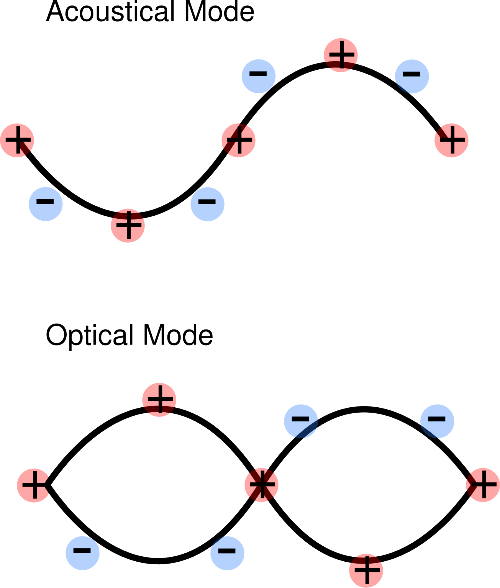
\includegraphics[width=\linewidth]{Figures/phonon-warwick-acoustic-optical-diagram.png}
  \caption[PHONON TYPE DIAGRAM]{STOLEN FROM UNI WARWICK https://warwick.ac.uk/fac/sci/physics/current/postgraduate/
  regs/mpagswarwick/ex5/phonons/}
  \label{fig:phonon_diagram}
\end{figure}

(((IS THIS STUFF CORRECT???))) Acoustic phonons are propagated by atoms displaced in-phase from their equilibrium positions, generating forces on their neighbours and thus subsequent displacement. Optical phonons are propagated by the opposite motion of adjacent positive and negatively-charged ions (conserving momentum, the lighter atom moves further). This motion is generated from the electric fields of external electromagnetic radiation ((OR DOES MOTION GENERATE EM FIELD?)), and is typically of a higher energy than its acoustic counterpart. 

Similar to how photons have wave particle duality, phonons are known as quasiparticles. This is useful for explaining how phonons waves interact with structural discontinuities and in phonon-phonon collisions. As a particle, a phonon is a quantised packet of vibrational energy. Unlike electronic heat conduction, there is a net motion of phonon particles from hot to cold regions. 

A phonon's mean free path (MFP) is the average distance it travels before scattering. The further the average phonon travels, the more efficient the heat transport and thus higher the thermal condutivity. A number of effects cause phonons to scatter: (1) collisions with other phonons in the lattice, (2) boundaries or defects in the material, and (3) impurities in the atomic structure. The MFP can be determined via Matthiessen's rule, which states the total thermal resistivity (inverse of conductivity) is equal to the sum of individual resistivities,
%
\begin{equation}
\frac{1}{\kappa} = \frac{1}{\kappa_{\mathrm{ph}}} + \frac{1}{\kappa_{\mathrm{b}}} + \frac{1}{\kappa_{\mathrm{d}}}\ ,
\end{equation}
%
where \textbf{ph}onon, \textbf{b}oundary, and \textbf{d}efect scattering effects are considered. The distance a phonon travels is proportional to conductivity, thus inversely proporitional to resistivity. The shorter the phonon path of an effect, the more it influences and contributes to, or detracts from, the MFP. This is displayed in the equation, where the inverse of the smallest number contributes the most to the sum.






%---------------------------------------
\subsection{What affects it?}
%---------------------------------------

Lattice thermal conductivity can be expressed in the form 
%
\begin{equation}
\kappa_{\mathrm{lat}} = \frac{1}{3} C_{\mathrm{v}} v l\ ,
\label{eq.cvvl}
\end{equation}
%
where $C_{\mathrm{v}}$ is the volumetric heat capacity, $v$ is the acoustic phonon velocity, and $l$ is the phonon mean free path.


%-------------------
\subsubsection{Pressure}
%-------------------

Volume of the material decreases with increasing pressure, with increasing depth into the Earth. This tends to increase the bulk and shear moduli, causing the seismic wave velocity, and thus the acoustic phonon velocity, to increase. Referring back to Eq.~\ref{eq.cvvl}, increasing pressure causes a conductivity increase.

%-------------------
\subsubsection{Temperature}
%-------------------

The phonon MFP increases with the volumetric heat capacity, until the saturation and convergence of this parameter at a material's Debye temperature (see Fig.~\ref{fig:debye-model}). Lattice conductivity is proportional to the MFP (Eq.~\ref{eq.cvvl}), so also increases with temperature up to the Debye limit. 

\begin{figure}[h!]
  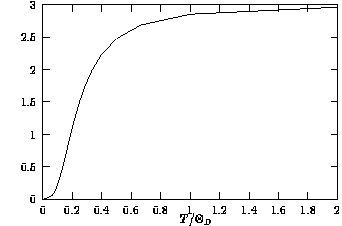
\includegraphics[width=\linewidth]{Figures/debye-model.png}
  \caption[DEBYE MODEL]{http://borisv.lk.net/matsc597c-1997/systems/Lecture4/node4.html}
  \label{fig:debye-model}
\end{figure}

Phonon-phonon scattering occurs as long as there are phonons, the effect of which increases with temperature past the Debye temperature. Conductivity change is inversely proporitional to temperature at this point, decreasing, and eventually saturating (see Fig.~\ref{fig:kappa-temp-dep}), to a minimum value as the MFP reaches its minimum (on the order of atomic spacing). Bridgmanite is above its Debye temperature for all lower mantle conditions I will consider. I can safely assume its conductivity will decrease with rising temperature.

\begin{figure}[h!]
  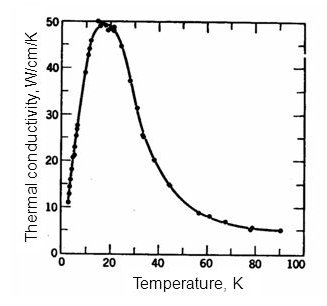
\includegraphics[width=\linewidth]{Figures/kappa-temp-dep.png}
  \caption[KAPPA AGAINST TEMP]{https://slideplayer.com/slide/9699097/31/images/29/
  Thermal+Conductivity+Metals+Dielectrics+Wiedemann-Franz+law\%3A.jpg}
  \label{fig:kappa-temp-dep}
\end{figure}


%-------------------
\subsubsection{Composition}
%-------------------

Considering a ``pure'' material, like \mgsios \bdg, the two sources of scattering are phonon-phonon, and phonon-boundary. Addition of impurities, such as in \mgfesios \pv, introduces phonon-impurity scattering and can reduce conductivity (refer back to Eq.~\ref{eq.cvvl}). The effect of impurities is less significant at high temperatures, when conductivity is already reduced by phonon-phonon sacttering. When the phonon-impurity path is much shorter than those of other scattering sources however, impurities can greatly reduce conductivity (via Matthiessen rule, above). Because of these relations, impurities will affect conductivity more higher in the mantle, with the effect reducing towards the CMB. The effect of impurities on thermal conductivity will be discussed extensively in CHAPTER FOUR.



%-----------------------------------------------------------
\section{Structure of the Earth}
%-----------------------------------------------------------
\label{sec:earth_structure}

\begin{figure}[h!]
  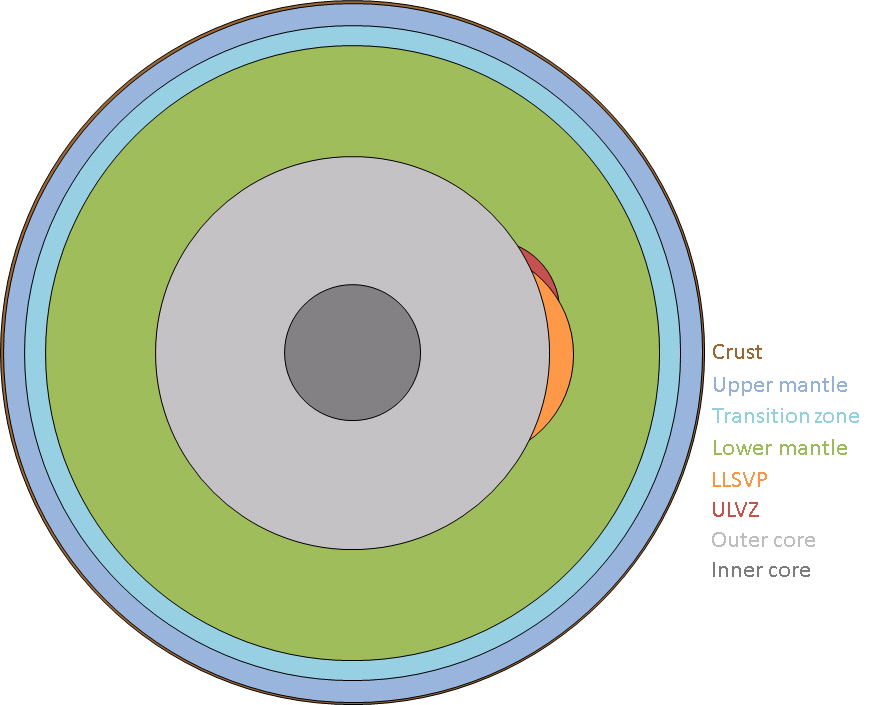
\includegraphics[width=\linewidth]{Figures/pp_earth_diagram.png}
  \caption[EARTH STRUCTURE DIAGRAM]{THE IDEA HERE IS FOR ME TO MAKE A FIGURE THAT INCLUDES ON THE MOST RELEVANT BITS OF THE EARTH, BASED OFF WHAT I MENTION IN FOLLOWING PARAGRAPHS. ADD SCALEBAR/DISTANCES? TEXT ON FIGURE? MARK CMB? MARK ATMOSPHERE/SURFACE?}
  \label{fig:earth_diagram}
\end{figure}

The average radius of the Earth is 6371~km, the properties of which change dramatically with depth to the centre. I will be focussed on the lower mantle, particularly the region close to the core (the core mantle boundary, CMB). Events in the lower mantle influence (and are influenced by) the upper mantle and lithosphere above, and the core below. Heat transport throughout the Earth is influenced by thermal conductivity, which in turn affects the dynamics of the system, the surface expression of this being plate tectonics. Heat flow also affects the core geodynamo, which produces the Earth's magnetic field. 

%---------------------------------------
\subsection{Lower mantle}
%---------------------------------------

The lower mantle encompasses the region after the mantle transition zone (660~km deep, $\sim$1900~K, $\sim$25~GPa) to the CMB (2900~km deep, $\sim$4000~K, 136~GPa). The composition of this region can be approximated as 75\% bridgmanite (MgSiO$_3$, magnesium silicate perovskite), 20\% periclase (MgO, magnesium oxide), and  5\% calcium silicate (CaSiO$_3$) perovskite \citep{Tronnes2009}. All of which are insulators and past their Debye temperatures at lower mantle conditions, with the potential for the inclusion of impurities such as iron and aluminium.

The exact nature of impurities is complicated to resolve, as there are a lot of variables. Iron comes in ferrous and ferric varieties, which can have varying electron spin states. The amount of iron is not partitioned evenly thoughout the mineral phases, periclase taking a larger proportion than bridgmanite for example. The nature of partitioning changes with physical conditions, where \ppvs may behave differently to \bdg.

A popular opinion is that bridgmanite is stable in the lower mantle until the bottom few 100~km, where it undergoes a pressure-driven phase change to post-perovskite \citep{Murakami2004,Oganov2004}. In places, close proximity to the CMB might transform post-perovskite back to perovskite structure due to the increased temperature. This ``double crossing'' of the bridgmanite stability range can be imaged seismically, where lens-like bands of post-perovskite are shown to pinch out laterally \citep{Lay2006}.

The lower mantle is not heterogeneous, with large-scale features around the CMB. Two large low shear velocity provinces (LLSVPs) can be found roughly underneath Africa and the Pacific. An associated feature is the ultra-low velocity zones (ULVZs), identified around the edges of LLSVPs. These can be observed seismically, but the reason they exist is unclear. It is suggested they are ``thermo-chemical features'', hotter and denser than the regular lower mantle. Increasing temperature and density tend to reduce seismic velocity, with increased density to offset the additional buoyancy from raised temperature. ``Thermo'' intuitively refers to the change in temperatures, while ``chemical'' changes are required to explain density increase. As a result, thermal conductivity will vary within these regions. Adding impurities such as iron would be a possible cause for density increase, such that the conductivity change should be quantified.

%---------------------------------------
\subsection{Lithosphere and upper mantle}
%---------------------------------------

The lithosphere (from 0~km depth) and upper mantle lie above the transition zone (to 660~km depth), which marks the top of the lower mantle. Although the chemistry of these regions is similar to that of the lower mantle, the physical conditions and mineral phases are different. Eruptive and subductive behaviour associated with plate tectonics is perhaps the most obvious consequence of mantle dynamics at the Earth's surface, and generally to humanity.

The ``rocky'' portion of the Earth (from the surface down to CMB) is largely some form of silicate mineral, often with magnesium and iron. The two main mineral transitions from the Earth's surface to the top of the lower mantle are pyroxene to garnet (40\%), and olivine through wadsleyite to ringwoodite \citep[60\%][]{Tronnes2009}. The olivine to wadsleyite change occurs at 410~km, marking the top of the mantle transition zone. Wadsleyite transitions to ringwoodite through this zone until 660~km, at which point it breaks down into lower mantle bridgmanite and ferropericlase.

%---------------------------------------
\subsection{Inner and outer core}
%---------------------------------------

The region beyond the CMB (starts at 2900~km depth) includes the core, comprised of its outer and inner sections. The liquid outer core extends to 5100~km depth, where the pressure-driven transition to solid inner core occurs. The composition of the core is dominated by iron, with various light elements suggested as possible alloying components.

Relative to the lower mantle, the outer core is a vigorously convecting system, and the core-side CMB can be considered to be an isothermal boundary. The main relevance to the lower mantle is the heat transfer across the CMB, the rate of which depends on the mantle conductivity and temperature. A second concern is that of chemical transfer between core and mantle, where iron from the core would be swapped various light mantle elements. Fe-content may increase in the lower mantle with CMB proximity, which in turn affects conductivity and the temperature profile for CMB heat flux.





%-----------------------------------------------------------
\section{Previous work - geophysics}
%-----------------------------------------------------------

%---------------------------------------
\subsection{STUFF THAT IS INFLUENCED BY CONDUCTIVITY}
%---------------------------------------
\label{sec:ch1:cond_in_earth}

Thermal conductivity in the deep Earth influences dynamic processes such as mantle convection and heat loss from the core \citep{Lay2008}. In this section I will discuss the prominent thermal conductivity-dependent processes.

%-------------------
\subsubsection{Mantle dynamics}
%-------------------

In the lower mantle \tcs changes with pressure, temperature, and composition, influencing features on a large scale. For example, \citet{Naliboff2006} used numerical models of mantle convection to show size and stability of convective plumes are sensitive to thermal conductivity above the core mantle boundary (CMB).

\citet{Dubuffet2000} investigated the effects of temperature and pressure-dependent \tcs on mantle convection, finding that depth-dependent \tcs encouraged heat transport via convective plumes. Compared to a constant conductivity model, vertical heat transfer was concentrated to these ``pipe-like'' structures, despite the horizontally-averaged heat flow for both systems being around the same value. Variable conductivity, even in one dimension, increased the spatial and temporal stability of convection. Plumes were thicker, had heads of larger surface area, and were hotter, compared to the uniform conductivity mantle model.

%-------------------
\subsubsection{Heat flow}
%-------------------

The most accessible estimate of the Earth's energy is the total heat flow at the surface, of which a value of $46\pm3$~TW is accepted as the upper bound. Sources of surface heat flow include; radiogenic heating ($20\pm3$~TW), mantle cooling (8--28~TW), and the conduction of heat across the CMB from core cooling \citep{Lay2008}. Conductive heat flow is constrained by thermal conductivity, a model of which is not available for all Earth conditions.

Better constraints on thermal conductivity are required to estimate CMB heat flow. This in turn would tell us more about the temperatures either side of the CMB, as well as the presence and nature of the lower mantle thermal boundary layer (TBL). Employing the most commonly used value for lower mantle conductivity, 10~\wmk~\citep{Lay2008}, heat flow across the CMB is expected to be 5--13~TW~\citep{Lay2008}. The value of 10~\wmks used by \citet{Lay2006} is an estimate of lowermost mantle \tc, based on extrapolation of a measurement at ambient conditions \citep{Osako1991}. Both higher and lower values have been proposed \citep[4--16~\wmk,][]{Manthilake2011}, illustrating how poorly constrained thermal conductivity is at CMB-relevant pressure/temperature conditions.

%-------------------
\subsubsection{Geomagnetism}
%-------------------

Using shear wave velocity as a proxy for CMB heat flow, \citet{Gubbins2007} showed that variations in mantle temperature gradients above the CMB can influence Earth's geodynamo. The present day magnetic field at the surface has four lobes, and these align above regions of fast shear wave velocity on the CMB. Ignoring compositional effects in the mantle, seismically-fast regions can be assumed to be cold. Considering Fourier's law (CITE), colder regions facilitate larger heat flows through steeper temperature gradients from the isothermal CMB.

\citet{Gubbins2007} recreate the geomagnetic observation of the aforementioned lobes using a core geodynamo simulation, where the upper boundary (CMB, lowermost mantle bottom) condition was a laterally varying heat flux. Knowing the \tc, especially as it changes with temperature, would better constrain mantle boundary conditions used in this and similar core dynamics models \citep{Ammann2014}.



%---------------------------------------
\subsection{DETERMINATIONS OF TC FOR EARTH MATERIALS/CONDITIONS}
%---------------------------------------

A range of atomic scale simulation methods are available to determine the lattice thermal conductivity of materials. These are invaluable for calculating thermal conductivity at conditions of which experiments are difficult, i.e. the extreme conditions found in the Earth's lower mantle (pressures and temperatures up to 136~GPa and 4000~K at the core-mantle boundary). 

Many studies assume lowermost mantle thermal conductivity to be 10~\wmk\ \citep[e.g.][]{Lay2008}, but uncertainty in the extrapolation of experimental results made at low pressures and temperatures gives a range of 4--16 \wmk~\citep{Brown1986, Osako1991, Hofmeister1999, Goncharov2009, Manthilake2011, Ohta2012}. 

The significance of radiative thermal conductivity, the transport of heat by photonic processes, is poorly constrained in the lower mantle. Until proven otherwise, it is convenient to assume the radiative component is small compared to the lattice component. The two components can simply be added to determine the total conductivity, a correction that can be applied to my results at a later date.

I give a review of experimental and computational determinations of conductivity for Earth-relevant conditions, where the Direct and Green-Kubo calculation methods are elaborated later on in Section REF (somewhere in chap2).

%-------------------
\subsubsection{Experiments}
%-------------------

There have been several computational studies to calculate the lattice thermal conductivity of bridgmanite at CMB conditions. \citet{Osako1991} measured the lattice thermal conductivity of MgSiO$_3$ perovskite, using a modified \AA ngstrom method. They investigated a temperature range of 160--340~K at ambient pressure. At 300~K, a conductivity of 5.1~\wmks was obtained. This value is reported by the authors to be consitent with chemical and structural analogues, MgSiO$_3$ enstatite (5.0~\wmk) and CaTiO$_{3}$ perovskite (4~\wmk). The authors extrapolated the value to mantle conditions, neglecting radiative thermal conductivity. They predicted a value of 3.0~\wmks just beneath the mantle transition zone at 1900~K, and 12.0~\wmks at the top of the \ddds layer at 2500~K, a four-fold increase. Thermal conductivity is highlighted as an important indictor of lowermost mantle structure, whether or not the \ddds layer can behave as a thermal boundary between core and mantle.

\citet{Manthilake2011} measured MgSiO$_3$ perovskite at 26~GPa and 473--1073~K, and periclase at 8 and 14~GPa between 373--1273~K. In order to estimate values of thermal conductivity at the top and bottom of D$^{\prime \prime}$ for a lower mantle compositional model of 4~perovskite~:~1~periclase, the authors extrapolated their measurements to high temperature and pressure. For an iron-free mantle, thermal conductivities of $18.9\pm1.6~$\wmks and $15.4\pm1.4$~\wmks are estimated for the top of D$^{\prime \prime}$ and CMB respectively. Similarly, for a mantle composition with Fe, thermal conductivities of $9.1\pm1.2$~\wmks and $8.4\pm1.2$~\wmks are calculated. This highlights the importance of impurities in controlling thermal conductivity in the lower mantle.

\citet{Ohta2012} measured the lattice thermal diffusivity of MgSiO$_3$ perovskite and post-perovskite at room temperature and pressures up to 144~GPa (using a diamond-anvil cell and light heating thermoreflectance). These results suggest a majority perovskite lowermost mantle would have conductivity of $\sim$11~\wmk, and that parts of the lowermost mantle where post-perovskite is stable will have a conductivity approximately 60\% higher. The authors suggest that these differences in conductivity between phases will not have a large effect on CMB heat flux, assuming the double-crossing perovskite phase model. The lattice conductivity of \mgsios perovskite is shown to increase with pressure and decrease with temperature as expected. The inclusion of impurities is expected to decrease lattice thermal conductivity.

%-------------------
\subsubsection{Calculations}
%-------------------

\citet{Haigis2012} used the Green-Kubo method (refer to REF) to calculate the lattice thermal conductivity of bridgmanite, post-perovskite, and periclase at lower mantle conditions. Assuming an iron-free composition with four parts bridgmanite to one part periclase, a model is constructed of density and temperature-dependent thermal conductivity along a geotherm. This model suggests great variation over the lower mantle, with a value of 9.5~\wmks at the top and 20.5~\wmks above \ddd. Based on the results of \citet{Manthilake2011}, \citeauthor{Haigis2012} suggest the inclusion of iron will lower thermal conductivity by up to half, bringing their result in line with \citet{Lay2006} ((10 WMK???)). The authors estimate the CMB heat flux to be 10.8~TW for an iron-bearing perovskite/periclase aggregate, dropping slightly to 10.6~TW for a similar post-perovskite aggregate. These values match other predictions of CMB heat flux \citep[e.g.][]{Lay2008}.

\citet{Dekura2013} used \ais anharmonic lattice dynamics with density functional theory (DFT) to calculate the lattice thermal conductivity of bridgmanite. At temperature of 300~K, they found conductivity increases from 9.8~\wmks at 23.5~GPa to 43.6~\wmks at 136~GPa. Temperature-dependence was found to be negative at 100~GPa, where conductivity decreases from 28.1~\wmks at 300~K to 2.3~\wmks at 4000~K. The pressure and temperature conditions used cover the entire range of accepted lower mantle conditions. From their results they calculated a Rayleigh number ($Ra$) of 10$^5$--10$^7$ for the mantle, in agreement with the geophysically-expected thermal convection (when $Ra < 10^3$--$10^4$). These results suggest that a CMB region at 136~GPa and 3200~K will have a conductivity of 5.3~\wmk, corresponding to a heat flux of 3--6~TW.

\citet{Ammann2014} used the direct method, a non-equilibrium molecular dynamics technique, to calculate the lattice thermal conductivity of bridgmanite and \ppvs under \ddds conditions. They found the conductivity of \ppv to be around 50\% larger than \bdg for the same conditions (12~\wmks compared to 8.5~\wmk). This relation is true even in the TBL, where increases in temperature reduce lattice conductivity for all \mgsios phases. An interesting result of their work is the observation of anisotropy for \ppvs conductivity. This may lead to a feedback mechanism, influence the formation and stability of convective plume structures.

\citeauthor{Ammann2014} also investigated the effects of impurities on conductivity, substituting magnesium with iron. They increase the mass of Mg atoms to resemble Fe, which tends to reduce conductivity. The lower mantle distribution of iron is not yet well-understood, specifically the partitioning between \bdg, \ppv, and periclase. Interestingly, the authors observed saturation in the conductivity reduction associated with atomic impurities, even for small Fe concentrations (see \ref{fig:ammann_sat}). Extrapolations of variable-composition experimental results must be applied carefully, increasing iron content past a certain point will not reduce conductivity any further.

\begin{figure}[h!]
  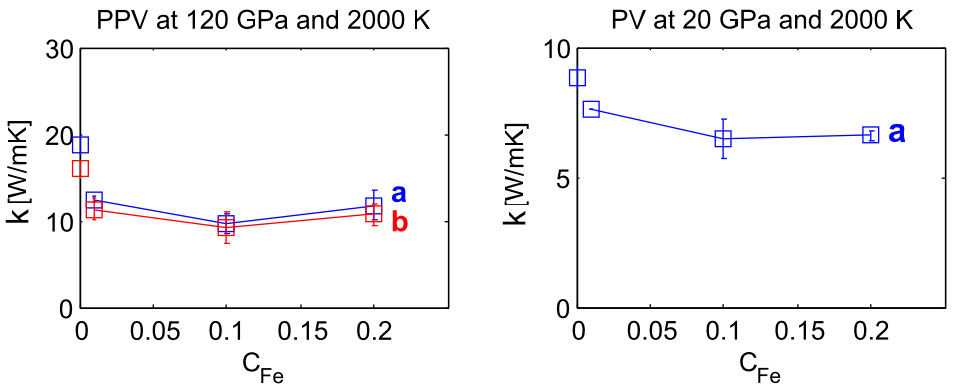
\includegraphics[width=\linewidth]{Figures/ammann_saturation.png}
  \caption[Thermal conductivity against Fe-content]{Thermal conductivity decrease due to inclusion of impurities is shown to saturate with increasing Fe-content, for \mgsios \ppv and perovskite phases. \textbf{a} and \textbf{b} refer to crystallographic directions along which conductivity was calculated. Figure modified from \citet{Ammann2014}.}
  \label{fig:ammann_sat}
\end{figure}

\citet{Tang2014} performed first-principles calculations to assess the \tcs of \mgsios
and the effect of Fe inclusions therein. These results feed into a model of conductivity along a lower mantle geotherm, of aggregate composition 4 \bdg : 1 periclase with 12.5\% Fe impurities. Their calculations model \mgfesios by increasing atomic mass, but not changing the force constants, in a manner similar to \citet{Ammann2014}. The inclusion of impurities has little effect at 136~GPa-4000~K, on the order of a few percent, but they note MgO is affected more considering its higher conductivity. The observation that conductivity is reduced less when it is already small due to the effect of temperature, matches the saturation described in \citet{Ammann2014}, but in turn disagrees with \citet{Haigis2012}. The uncertainity is large when experimental data is extrapolated, especially when considering the (temperature-dependent) effect of impurities.

\citet{Ghaderi2017} investigate the lattice conductivity of \bdgs using ab initio lattice dynamics calculations, considering a range of pressures at room temperature (mirroring previous experimental measurements). \mgsios conductivity is found to increase from 10.7~\wmk at 0~GPa, to 59.2~\wmk at 100~GPa. Conductivity is extrapolated to lower mantle conditions and determined for a sample geotherm. The value initially increases with depth as the effect of increasing pressure dominates, until around 400~km above the CMB, where temperature effects take over and conductivity reduces. A value of $\sim$5.2~\wmk for CMB conditions of 136~GPa and 4000~K. 

The authors also discuss anisotropy, after observing differences of $\sim$25\% between the most ($\kappa_{\mathrm{zz}}$) and least ($\kappa_{\mathrm{xx}}$ and $\kappa_{\mathrm{yy}}$, depending on pressure) conductive crystallographic directions. This observation is similar to that from \citet{Ammann2014}.

The concept of a minimum phonon mean free path is discussed by \citet{Ghaderi2017}, the idea that a minimum MFP causes conductivity to saturate at high temperatures, showing a dependence different to the expected $1/T$. The authors suggest an explanation for this phenomena, which is radiative heat transport. The cause of low MFP is called into question, whether it be small group velocities, or short phonon lifetimes. In any case, the authors assume the minimum MFP to not be correct, and extrapolate to high temperatures with a $1/T$ relation.

%-------------------
\subsubsection{Radiative conductivity}
%-------------------
\label{sec:rad_cond}

\citet{Hofmeister1999} produced a model of thermal conductivity for the entire mantle using data from infrared reflectivity methods. The radiative component at maximum was found to be small compared to the lattice conductivity, between 10--15\% depending on the geotherm model used. This corresponds to radiative conductivity values of 0.67--0.82~\wmks compared to 5.8--6.7~\wmks for the total conductivity at the top of \ddd.

\citet{Keppler2008} studied the near-infrared and optical absorption spectra of silicate perovskite up to pressures of 125~GPa at room temperature. From both their tests and visual inspection, it can be shown that their synthesised perovskite remains transparent at high pressures. Extrapolating their results to high temperatures (4500~K) they suggest that the maximum radiative thermal conductivity above the CMB is around 10~\wmk, implying that radiative conductivity is likely to be an important component of the total conductivity at lower mantle conditions. The study does not measure the variation of absorption spectra with temperature and pressure, of which experimentation is currently unfeasible.

\citet{Goncharov2008} performed a similar optical absorption spectra analysis up to 133~GPa, but with the opposite conclusion to \citet{Keppler2008}. They agreed the radiative conductivity was dependent on the amount, redox state, and spin state of iron, but disagreed with its significance. \citet{Goncharov2008} estimated radiative conductivity would not exceed 0.54~\wmks at the top of the \ddds layer, a value in line with \citet{Hofmeister1999} and at odds with \citet{Keppler2008}. 

\citet{Tang2014} re-evaluated the works of \citet{Keppler2008} and \citet{Goncharov2008} to create a profile of radiative conductivity in the lower mantle. \citeauthor{Tang2014}'s profile suggests that the previous works have a more reasonable agreement than they show, using analysis which gives an upper bound on the conductivity. Radiative heat transfer is inhibited in the same way as conductive, by impurities and grain boundaries which are not considered when calculating this upper bound. Unlike lattice thermal conductivity, radiative conductivity increases with temperature, steeply so in the mantle thermal boundary layer. When the opposing temperature dependencies of lattice and radiative conductivity are considered in tandem, they suggest that the thermal conductivity of the lower mantle is largely temperature-independent above the \ddds region at around 3~\wmk. Thermal conductivity is found to increase to 5.5 \wmks in the TBL, due to the increased significance of the radiative component.

More recently, \citet{Lobanov2017} determine the radiative conductivity of \ppvs ($1.2\pm0.2$~\wmk, 10\%~Fe), \bdgs ($2.2\pm0.4$~\wmk, 10\%~Fe), and ferropericlase ($0.2\pm0.1$~\wmk, 15\%~Fe). They measure optical absorption from diamond anvil cell experiments, extrapolating radiative conductivity from absorption coefficients to lower mantle conditions ($\sim$130~GPa, 4000~K). While they model radiative conductivity generally increasing towards the CMB, it decreases from \bdgs to \ppv. Ferropericlase is found to be less radiative than either of the \mgfesios phases, with all of the considered minerals having higher lattice conductivities compared to radiative. The authors conclude by suggesting that the lattice conductivity will decrease faster than radiative with the inclusion of Fe-impurities, changing the relative significance from low to high Fe content. The results from this study agree with the previous works, that radiative heat transport is not the dominant process in the lower mantle compared to lattice conductivity, but it cannot be ignored however.

\begin{sidewaystable}[ph!]
\centering
\newcolumntype{P}{ >{\centering\arraybackslash} m{1.5cm} }
\newcolumntype{T}{ >{\centering\arraybackslash} m{1.4cm} }
\newcolumntype{K}{ >{\centering\arraybackslash} m{2.4cm} }
\caption[CONTENTS CAPTION]{THIS TABLE IS NOT UPDATED FOR GHADERI OR LOBANOV. Comparison of previous lower mantle thermal conductivity values.}
\vspace{2mm}
  \begin{tabular}{ | c | c | c | P | T | K | c | }
	 \hline
	
	Paper & Type & Material & Pressure (GPa) & Temp. (K) & Thermal Conductivity (\wmk) & Notes  \\ \hline \hline

	\multirow{5}{*}{\parbox{2.2cm}{\cite{Osako1991}}} & \multirow{5}{*}{Experiment} & \mgsios perovskite & 0 & 300 & 5.1 & \multirow{3}{*}{\parbox{2.5cm}{Measurement, w/ analogues}} \\ \cline{3-6}
 	& & \mgsios enstatite & 0 & 300 & 5.0 &  \\ \cline{3-6}
 	& & CaTiO$_3$ perovskite & 0 & 300 & 4 &  \\ \cline{3-7}
 	& &  \multirow{2}{*}{\mgsios perovskite} & 24 & 1900 & 3 & \multirow{2}{*}{Extrapolation} \\ \cline{4-6}
 	& & & 127 & 2500 & 12 & \\ \hline \hline
 	
% 	\multirow{4}{*}{\parbox{2.2cm}{\cite{Manthilake2011a}}} & \multirow{4}{*}{Experiment} & \multirow{2}{*}{CaGeO$_3$ perovskite} & 127 & ? & 3.3 & \multirow{4}{*}{\parbox{2.5cm}{Extrapolation}} \\ \cline{4-6}
% 	& & & 136 & ? & 2.2 & \\ \cline{3-6}
% 	& & \multirow{2}{*}{\parbox{4cm}{4 CaGeO$_3$ perovskite : 1 MgO periclase}} & 127 & ? & 6.4 & \\ \cline{4-6}
% 	& & & 136 & ? & 4.5 & \\ \hline \hline

	\multirow{4}{*}{\parbox{2.8cm}{\cite{Manthilake2011}}} & \multirow{4}{*}{Experiment} & \multirow{4}{*}{4 \mgsios pv : 1 periclase} & 127 & 2600 & 9.1 $\pm$ 1.2 & \multirow{2}{*}{\parbox{3cm}{Extrap., mantle model (w/ Fe)}} \\ \cline{4-6}
	& & & 136 & 4100 & 8.4 $\pm$ 1.2 & \\ \cline{4-7}
	& & & 127 & 2600 & 18.9 $\pm$ 1.6 & \multirow{2}{*}{\parbox{3cm}{Extrap., mantle model (no Fe)}} \\ \cline{4-6}
	& & & 136 & 4100 & 15.4 $\pm$ 1.4 & \\ \hline \hline
 	
 	\multirow{4}{*}{\parbox{2.2cm}{\cite{Ohta2012}}} & \multirow{4}{*}{Experiment} & \mgsios perovskite & \multirow{4}{*}{136} & \multirow{4}{*}{3700} & 9.0 $\pm$ 1.6 & \multirow{4}{*}{\parbox{2.5cm}{Extrapolation}} \\ \cline{3-3} \cline{6-6}
 	& & \mgsios post-perovskite & & & 16.8 $\pm$ 3.7 & \\ \cline{3-3} \cline{6-6}
 	& & 4 \mgsios pv : 1 periclase & & & 11.0 $\pm$ 2.0 & \\ \cline{3-3} \cline{6-6}
 	& & 4 \mgsios ppv : 1 periclase & & & 17.8 $\pm$ 3.9 & \\ \hline \hline
 	
 	 \multirow{6}{*}{\parbox{2.2cm}{\cite{Haigis2012}}} & \multirow{6}{*}{\parbox{2.3cm}{Green-Kubo Calculation}} & \multirow{2}{*}{4 \mgsios pv : 1 periclase} & 24 & 2200 & 9.5 & \multirow{2}{*}{Calculation} \\  \cline{4-6}
 	 & & & 127 & 2900 & 20.5 & \\ \cline{3-7}
 	 & & Pv/periclase aggregate & \multirow{4}{*}{136} & \multirow{4}{*}{3739} & 16.4 $\pm$ 2.7 & \multirow{4}{*}{\parbox{2.6cm}{Extrapolation, mantle model}} \\  \cline{3-3} \cline{6-6}
 	 & & Ppv/periclase aggregate & & & 16.6 $\pm$ 2.7 & \\  \cline{3-3} \cline{6-6}
 	 & & Pv/periclase aggregate w/ Fe & & & 8.2 & \\  \cline{3-3} \cline{6-6}
 	 & & Ppv/periclase aggregate w/ Fe & & & 8.3 & \\ \hline \hline
 	 
 	 \multirow{5}{*}{\parbox{2.2cm}{\cite{Dekura2013}}} & \multirow{5}{*}{\parbox{2cm}{Lattice Dynamics}} & \multirow{5}{*}{\mgsios perovskite} & 23.5 & 300 & 9.8 & \multirow{4}{*}{Calculation} \\ \cline{4-6}
 	 & & & 136 & 300 & 43.6 & \\ \cline{4-6}
 	 & & & 100 & 300 & 28.1 & \\ \cline{4-6}
 	 & & & 100 & 4000 & 2.3 & \\ \cline{4-7}
 	 & & & 136 & 3200 & 5.3 & Extrapolation \\ \hline \hline
 	 
 	 \multirow{2}{*}{\parbox{2.2cm}{\cite{Ammann2014}}} & \multirow{2}{*}{\parbox{2.3cm}{Direct method}} & \mgsios perovskite & \multirow{2}{*}{136} & \multirow{2}{*}{3739} & 8.5 & \multirow{2}{*}{Calculation} \\ \cline{3-3} \cline{6-6}
 	 & & \mgsios post-perovskite & & & 12 & \\ \hline \hline
 	 
 	 \multirow{3}{*}{\parbox{2.2cm}{\cite{Tang2014}}} & \multirow{3}{*}{\parbox{2.3cm}{Peierls Boltzmann}} & \multirow{3}{*}{4 \mgsios pv : 1 periclase} & 24 & 2000 & 2.5 & \multirow{3}{*}{\parbox{2.5cm}{Including Fe, with radiative}} \\ \cline{4-6}
 	 & & & 127 & 3000 & 3.5 & \\ \cline{4-6}
 	 & & & 136 & 4000 & 5.5 & \\ \hline
 	
 	
 	
 	
	\end{tabular}
\label{tab:summary}  

\end{sidewaystable}
\pagebreak

%-----------------------------------------------------------
\section{Thesis outline}
%-----------------------------------------------------------

!!! I SAY ``i'' ALOT, I DO THIS, I DO THAT

In this Chapter, I introduced the concepts surrounding thermal conductivity generally and in the deep earth. A great deal of uncertainty surrounds this parameter at those conditions, which I explore in subsequent chapters.

In Chapter \ref{Chapter2}, I provide an overview of the methods and expand on issues. I outline my computational approaches, for the non-equilibrium molecular dynamics direct method and equilibrium molecular dynamics Green-Kubo method. I show convergence of computed conductivity with respect to simulation time and physical conditions.

In Chapter \ref{Chapter3}, I investigate the effect of system size and shape on the converged, computed conductivities. By comparing and contrasting methodologies, I am able to establish the requiste system properties to obtain accurate results at a given condition. This leads me to analyse previous works, and suggest results which may not be correct due to effects of simulation size.

In Chapter \ref{Chapter4}, I apply my converged computational techniques to investigate the effect of introducing Fe impurities into \bdg, and how this affects the resultant conductivity across the enitre endmember suite. Furthermore the effect is constrained across multiple lower mantle temperatures, allowing me to create a model of \mgfesios conductivity as a function of temperature.

In Chapter \ref{Chapter5}, I discuss the temperature and compositional-dependence on heat flow across the CMB, and the effect this has on the whole lower mantle. A review of findings will be presented with suggestions for future work, both in thermal conductivity computations and applications thereof to deep earth studies.



%---------------------------------------
\subsection{Aims}
%---------------------------------------

(The questions I answered)

%---------------------------------------
\subsection{Objectives}
%---------------------------------------

(The things I did)

\chapter{Computing thermal conductivity} 

\label{Chapter2} 

In Chapter~\ref{Chapter1}, I introduced the key concepts surrounding this study. I will be investigating the magnitude of thermal conductivity throughout the deep Earth, considering the effect of physical conditions and Fe impurities. I will be using computational approaches to access this parameter, as experiments are difficult to perfrom in the regime I require. 

Part of computing results is ensuring the simulations are running faithfully to the material of interest and the physical processes that operate in bulk materials. In this chapter I introduce the background to calculating conductivity through simulation, and show fundamental system setup and parameter convergence. 

The following chapters apply theory introduced here to investigate how conductivity is affected by; system shape and size, and adding impurities to an otherwise regular crystal structure.

%-----------------------------------------------------------
\section{Atomic-scale modelling}
%-----------------------------------------------------------

!!! THIS SECTION HAS REDUNDANCY WITH ABOVE CHAPTER INTRO SPIEL

!!! PROBABLY REVISE HEAVILY

Knowledge of thermal conductivity is important for modelling the deep earth, but can not be measured experimentally at core mantle boundary conditions. Atomic scale simulations sidestep experimental limitations, but system size must be chosen carefully in order to determine accurate conductivity values. 

A range of atomic scale simulation methods are available to determine the lattice thermal conductivity of materials. These are invaluable for calculating thermal conductivity at conditions of which experiments are difficult, e.g. the extreme conditions found in the Earth's lower mantle (pressures and temperatures up to 136~GPa and 4000~K at the core-mantle boundary). 

%---------------------------------------
\subsection{Computational approaches (for modelling atoms...?)}
%---------------------------------------

Before you can calculate material properties of interest, you need to determine how the atoms will interact with one another in your system. I do not mean the magnitude of the interactions or the parameters you choose to replicate a material, but the specific theoretical approach of atomic-scale modelling. There are multiple regimes for doing so, a couple of which are described below.

%-------------------
\subsubsection{Molecular dynamics}
%-------------------

In a moldecular dynamics (MD) calculation, atoms in a simulation cell have masses, velocities, and forces acting between them. At each computational timestep the net force on each atom is calculated from all the other atoms. Accelerations are then calculated from Newton's second law of motion, which are used to update the velocities and positions of the atoms. The process is repeated, iteratively updating parameters every timestep. At zero temperature, a parameter such as unit cell volume will converge, but this is not true when finite temperatures are considered. Temperature fluctuations mean cell volume will constantly change, regardless of simulation length. The solution is to take the cumulative average over many timesteps, which converges eventually.

!!! FLOWCHART FIGURE, MD TIMESTEP PROCESS?

%-------------------
\subsubsection{Lattice dynamics}
%-------------------

An alternative approach to MD is lattice dynamics (LD),where the response of all atoms to the motion of one is considered. Each atom in the simualtion cell is perturbed in turn, the motions and response of the other atoms stored  in a 3 by 3 tensor for each atom pairing. The tensor takes significant time to compute compared to a single MD timestep, but can be used to calculate various material properties once obtained. The focus of this study will be on MD approaches, but LD results from literature will be reviewed for comparison.

!!! ADD A REFERENCE AND FORGET ABOUT IT?

!!! DO I NEED TO SAY WHY I AM NOT USING LD? WHY AM I NOT USING LD!?














%---------------------------------------
\subsection{Calculating atomic interactions}
%---------------------------------------

!!! ADD INTRO SPIEL HERE

%-------------------
\subsubsection{Density functional theory}
%-------------------

Density functional theory (DFT) is a way of determining accurate interatomic forces. The properties of the electrons are considered along with the nuclei, which increases the computational cost and simulation run time. This additionally limits the size of systems, or number of atoms (on the order of thousands), that can be considered. Calculating from first principles in this manner should only be considered if you know the system parameters for converged results, and they can be completed on a suitable timescale. I will be opting for a different approach, as I wish to investigate a large amount of big systems systems, potentially for multiple compositional variations.

!!! ANY OTHER ALTERNATIVE APPROACHES THAT NEED TO GO HERE?

%-------------------
\subsubsection{Classical interatomic potentials}
%-------------------

The alternative to DFT is to use empirically-derived potentials to calculate the interatomic forces. Whereas calculating from first principles considers the interactions of atoms and their outer shell electrons, interatomic potentials use an approximation of the electronic potential component (i.e. a classical atomic model). 

Systems on the order of millions of atoms can be considered with atomic potentials, due to significantly reduced computational cost compared to DFT. The trade-off is accuracy however, which is controlled by the characteristics of the employed potential. These potentials are set up to reproduce a set of experimental results, but the is no certainty they reflect true values outside their calibrated range of conditions. A realsitic model reproduces the structural, elastic, and thermal properties of a material. A common feature of classical potentials is to underestimate the diagonal terms of the elastic constant tensor, and overestimate the off-diagonal, where the discrepancy increases with pressure \citep{Chen2012}.

%-------------------
\subsubsection{Oganov's \bdgs potential}
%-------------------

The interatomic potential I will be using  was developed by \citet{Oganov2000}. Many potentials exist for \mgsios perovskite, but the aforementioned is robust up to lower mantle pressures and temperatures. The interatomic potential function includes ionic, covalent, and van der Waals components. The dominant long-range term is the Coulomb interaction, and the short-range interactions are described using a Buckingham potential with the Born-Mayer potential, and a $C/r^{6}$ van der Waals term. The equation for pair-wise potential (summed for potential energy of the system) takes the form
%
\begin{equation}
V_{ij}^{\mathrm{Buck}}
= \frac{1}{4 \pi \epsilon_{0}} 
\frac{q_{i} q_{j}}{r_{ij}} 
+ b_{ij}\ exp\left ( \frac{-r_{ij}}{\rho_{ij}} \right )
- \frac{c_{ij}}{{r_{ij}}^{6}} \  ,
\label{eq.buck}
\end{equation}
%
where $q_{i}$ and $q_{j}$ are the charges of atoms $i$ and $j$, $r_{ij}$ is the distance between them, $b_{ij}$ is the pre-exponential repulsive parameter for the pair, $\rho_{ij}$ is the repulsion exponent, and $c_{ij}$ is the van der Waals parameter.
There are three sets of these paramters, for each of the interacting atomic pairs (shown in Table~\ref{tab.oganov}). The charges for Mg, Si, and O atoms are $1.9104$, $2.9043$, and $-1.6049$, respectively.
%
\begin{table}[h]
\centering
\caption[CONTENTS BIT]{\label{tab.oganov}Parameters used to define \citet{Oganov2000}'s \mgsios perovskite potential.}
\begin{tabular}{clll} 
Bond $ij$ & $b_{ij}$ (eV)  & $\rho_{ij}$ (\AA) & $c_{ij}$ (eV.\AA$^{6}$) \\ \hline
Mg-O        & 1041.435        & 0.2866                 & 0                \\
Si-O          & 1137.028        & 0.2827                 & 0                \\
O-O          & 2023.800        & 0.2674                  & 13.83         \\ \hline       
\end{tabular}
\end{table}



%-------------------
\subsubsection{SETTING UP POTENTIAL CUTOFFS}
%-------------------

Part of applying classical potentials is setting up the distance over which they act, the maximum seperation between two atoms before they are not paired for force calculation. Too small a cut-off distance, and the material is not being replicated faithfully. Too large a cut-off, you are performing more calculations than you need, and will increase computation time. The potential between two atoms is inversely proportional to their separation (see Eq. \ref{eq.buck}), ``cutting off'' in this manner is acceptable when the value is tending towards zero with large interatomic distance. I consider two cut-off distances, for both the Coulombic and the Buckingham interactions (the former have a larger value than the latter).

 !!! BUT WHAT DID I DECIDE ON THOUGH 











%---------------------------------------
\subsection{Finite-size effects}
%---------------------------------------

Computational techniques are not limited by the reproduction of physical conditions like experiments, this does not mean they are without limitations however. Finite-size effects refer to when the number of atoms or system shape and size affect the computed result, compared to an infinite system. In the case of thermal conductivity, the problem arises when phonons are truncated by boundaries in the simulation cell. As discussed in Chapter~\ref{sec.phonon_explan}, phonons have wave-like properties, including wavelength. 

When a simulation cell is shorter than a phonon, that phonon cannot be represented in the system. This will mean a calculation is tending to underestimate conductivity. The opposite scenario is also true, if the phonon mean free path is longer than the distance between boundaries in a system, phonon scattering behaviour is not being replicated accurately. This leads to overestimations, where phonons are able to transport heat unimpeded, and conductivity is strongly dependent on system size \citep{Tadano2014}. 

The FSE observed for a material change with thermal conductivity/phonon MFP, and thus are pressure, temperature, and composition sensitive. Long MFPs require larger systems to eliminate FSE (and vice versa) [[[BUT IS THIS TRUE?]]].

This can be a problem when employing DFT calculations, where systems sizes must be kept small to maintain computational efficiency. Testing system size is also a problem, as calculations of large systems must be performed to check convergence of results.

%-------------------
\subsubsection{LAMMPS}
%-------------------

LAMMPS (Large-scale Atomic/Molecular Massively Parallel Simulator) is a classical molecular dynamics code \citep{Plimpton1995}. I will be using it to look at large systems (up to the order of $10^5$ atoms) and assess how size and shape affects results. While calculations using interatomic poternials are not as accurate as those using DFT, a main focus of this work will be on the observations of conductivity magnitude change between systems of varying size. The \wmks result isn't as important as confirming phonon behaviour is not being greatly inhibited. 

While not considered here, the system size parameters I determine for \bdgs at a range of temperatures and pressures could be used in a DFT calculation. This ensures the DFT calculation is using a large enough arrangement of atoms, while providing a useful reliability check for my classical results. 

















\pagebreak
















%-----------------------------------------------------------
\section{Computing \tc}
%-----------------------------------------------------------

I will be using two approaches, both utilising classical interatomic potentials, to calculate thermal conductivity throughout this thesis. They will be explained later in this section, and are as follows,

(1) The non-equilbrium molecular dynamics-based ``direct method'', where thermal conductivity is calculated from an imposed heat flux and corresponding temperature gradient via Fourier's Law \citep{Muller-Plathe1997,Nieto-Draghi2013}.

(2) Equilibrium molecular dynamics based on the Green-Kubo relations to determine the thermal conductivity from heat flux fluctuations and their time-dependence \citep{Green1954,Kubo1957,Kubo1966,Schelling2002}. 


\citet{Stackhouse2010} review other methods to compute thermal conductivity, including the above but also,

(3) Anharmonic lattice dynamics \citep{Tang2009}. %(BTE)CHERNATYNSKIY and PHILLPOT 2010?

(4) Combined quasiharmonic lattice dynamics and molecular dynamics method \citep{DeKoker2009}.

!!! Fixed ends? Sinusoidal temperature perturbation?

The Green-Kubo and direct method use the same underlying atomic model, but calculate \tcs differently. They have their own unique system setup procedures, data processing work flows, and finite-size effects. In the following sections, each method will be considered individually, before a review of literature comparing the two, and how I will use them to analyse their FSE.



%---------------------------------------
\subsection{Direct method}
%---------------------------------------
The direct method is the computational implementation of a typical experiment to measure thermal conductivity, using Fourier's law to relate heat flux ($q$) and temperature gradient ($\nabla{T}$) to thermal conductivity ($k$), 
%
\begin{equation}
q=-k \nabla{T} 
\label{fourier}.
\end{equation}

%-------------------
\subsubsection{System setup}
%-------------------

In the direct method energy is transferred from one group of atoms to another, creating hot and cold regions between which heat flows. The resultant temperature gradient is measured by calculating the temperature of individual groups of atoms along the direction of the heat flux. Simulation cells tend to be long relative to their cross-sectional area, defined as height by width (see Figure~\ref{fig:cell_dia}). Cell boundaries are periodic and the hot and cold sections are half the cell length apart, meaning heat flows in both directions from hot to cold (one of which is across the length-end periodic boundary). This results in two similar temperature gradients which can be averaged.

\begin{figure}[h]
  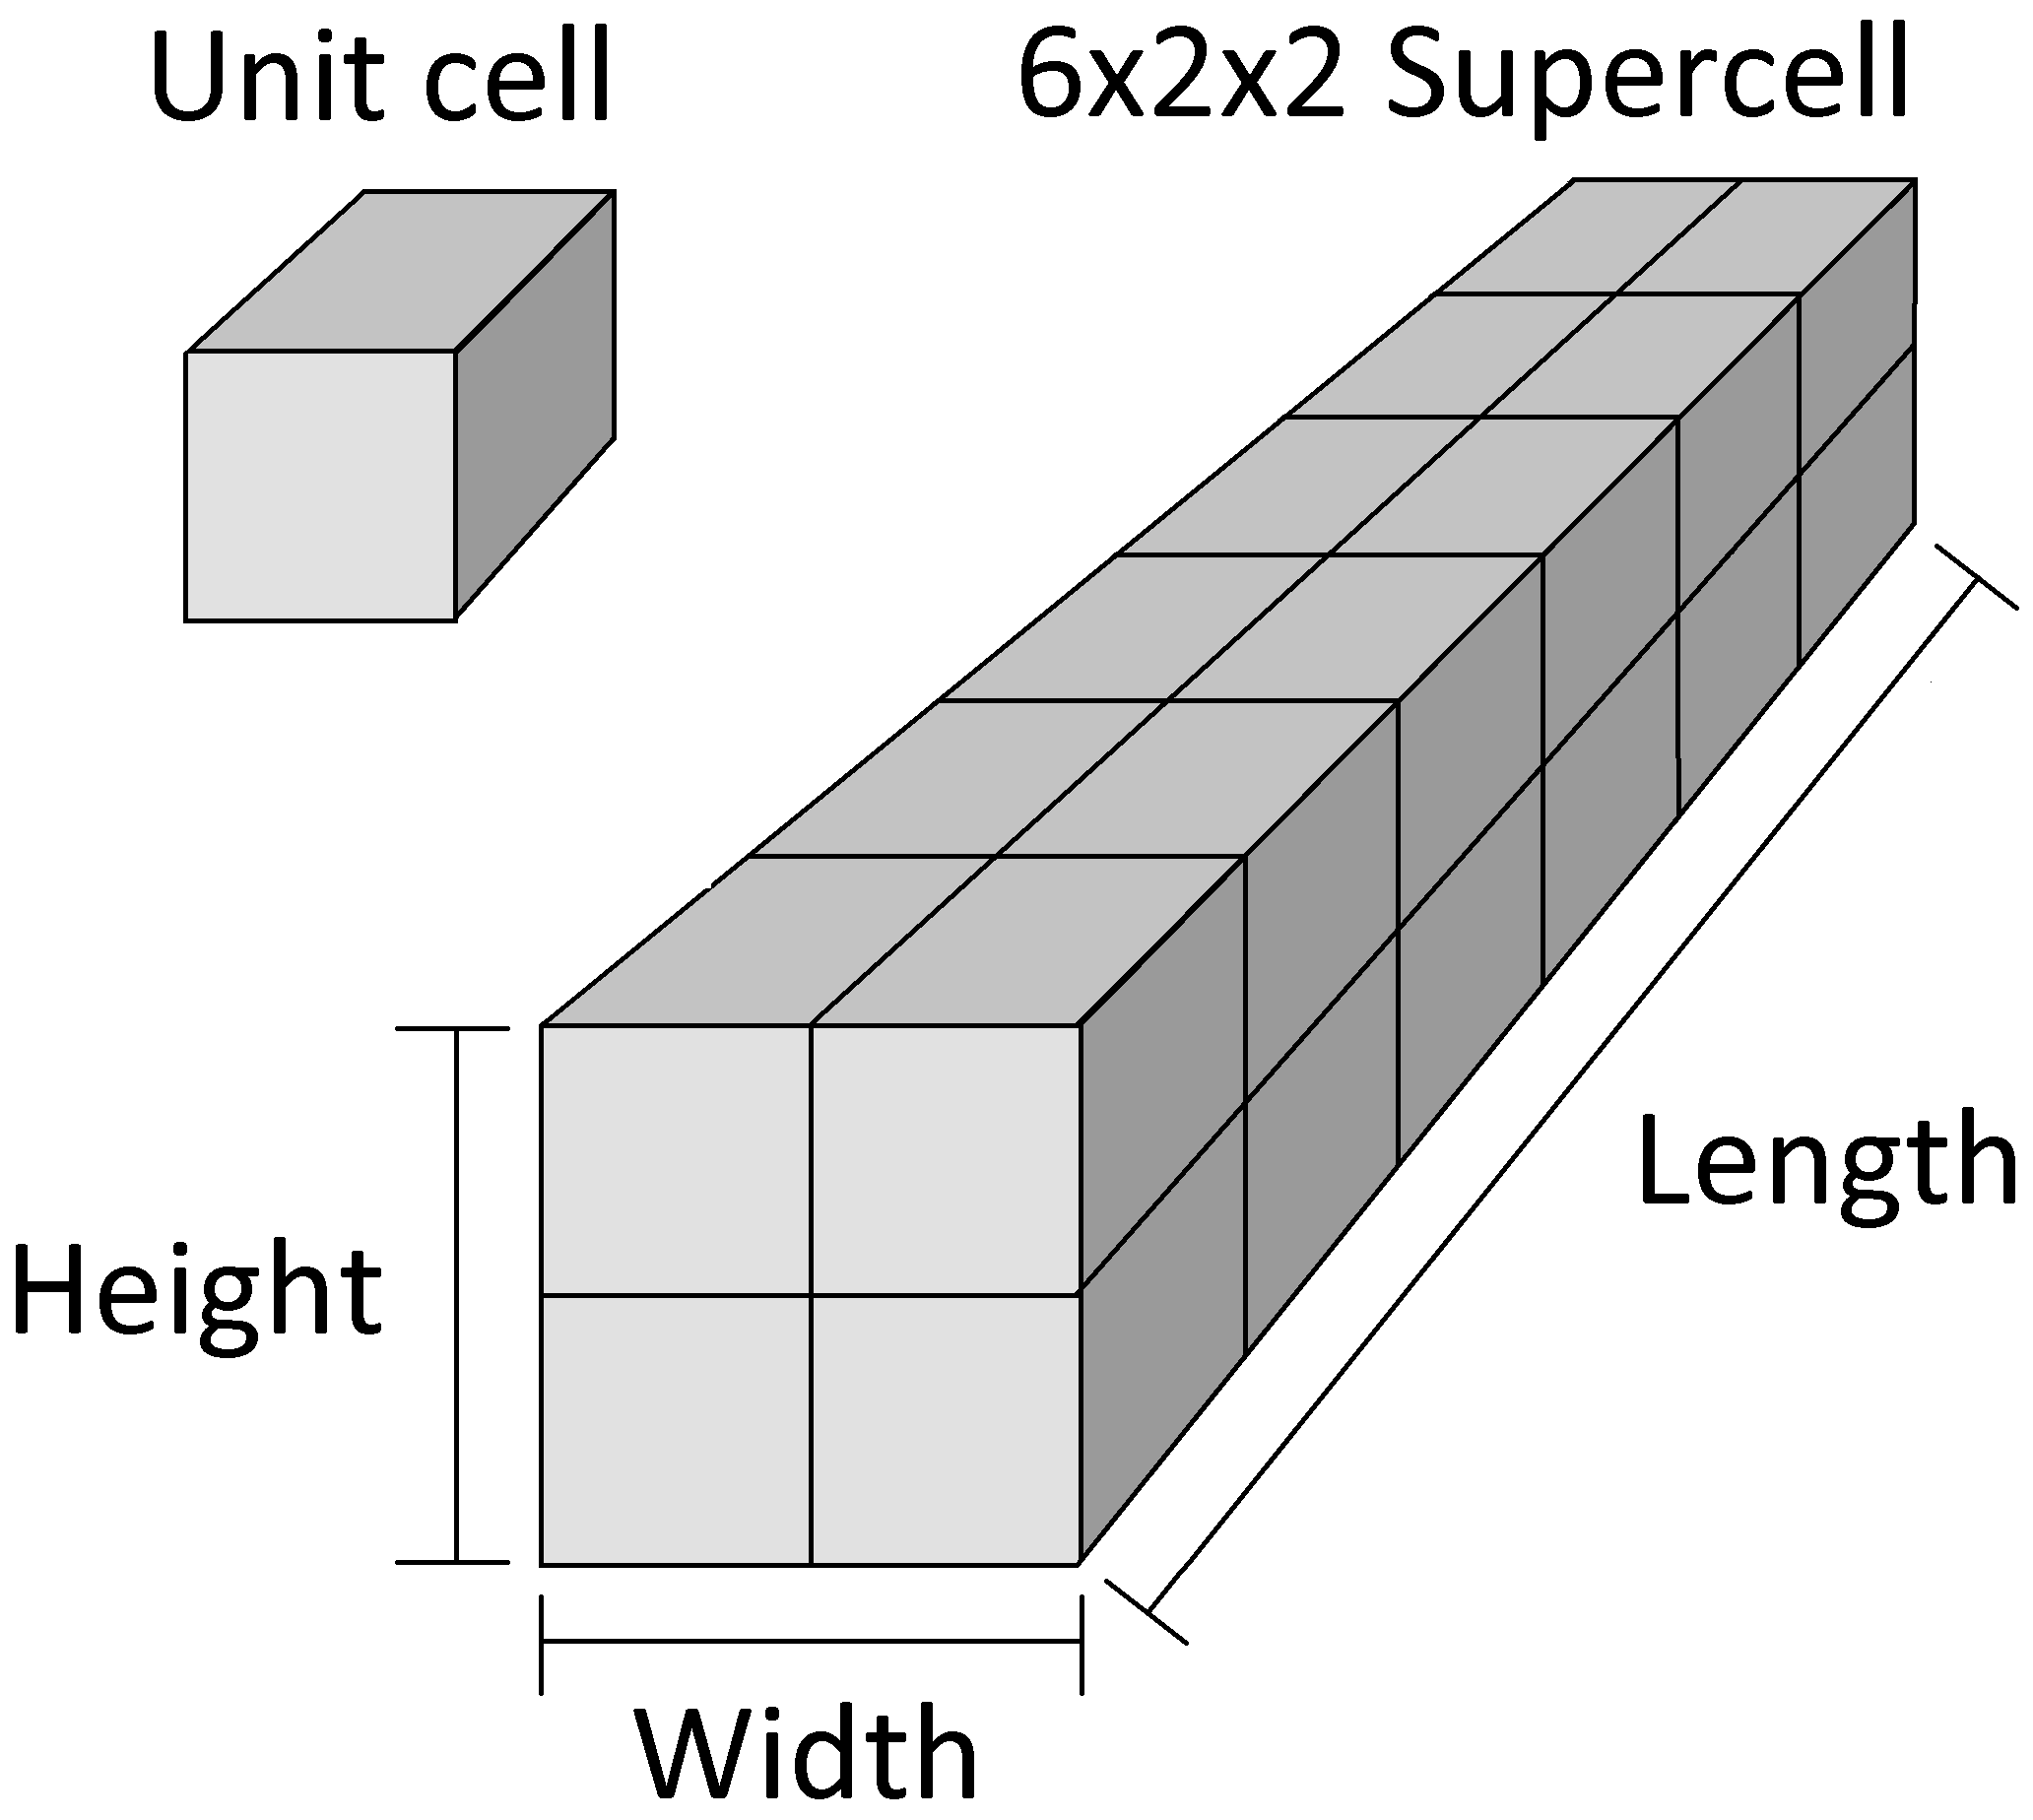
\includegraphics[width=\linewidth]{Figures/cell_diagram.png}
  \caption{The unit cell represents the smallest box of atoms that can be replicated to produce a crystal structure. A supercell is an arrangement of unit cells.}
  \label{fig:cell_dia}
\end{figure}

\begin{figure}[h]
  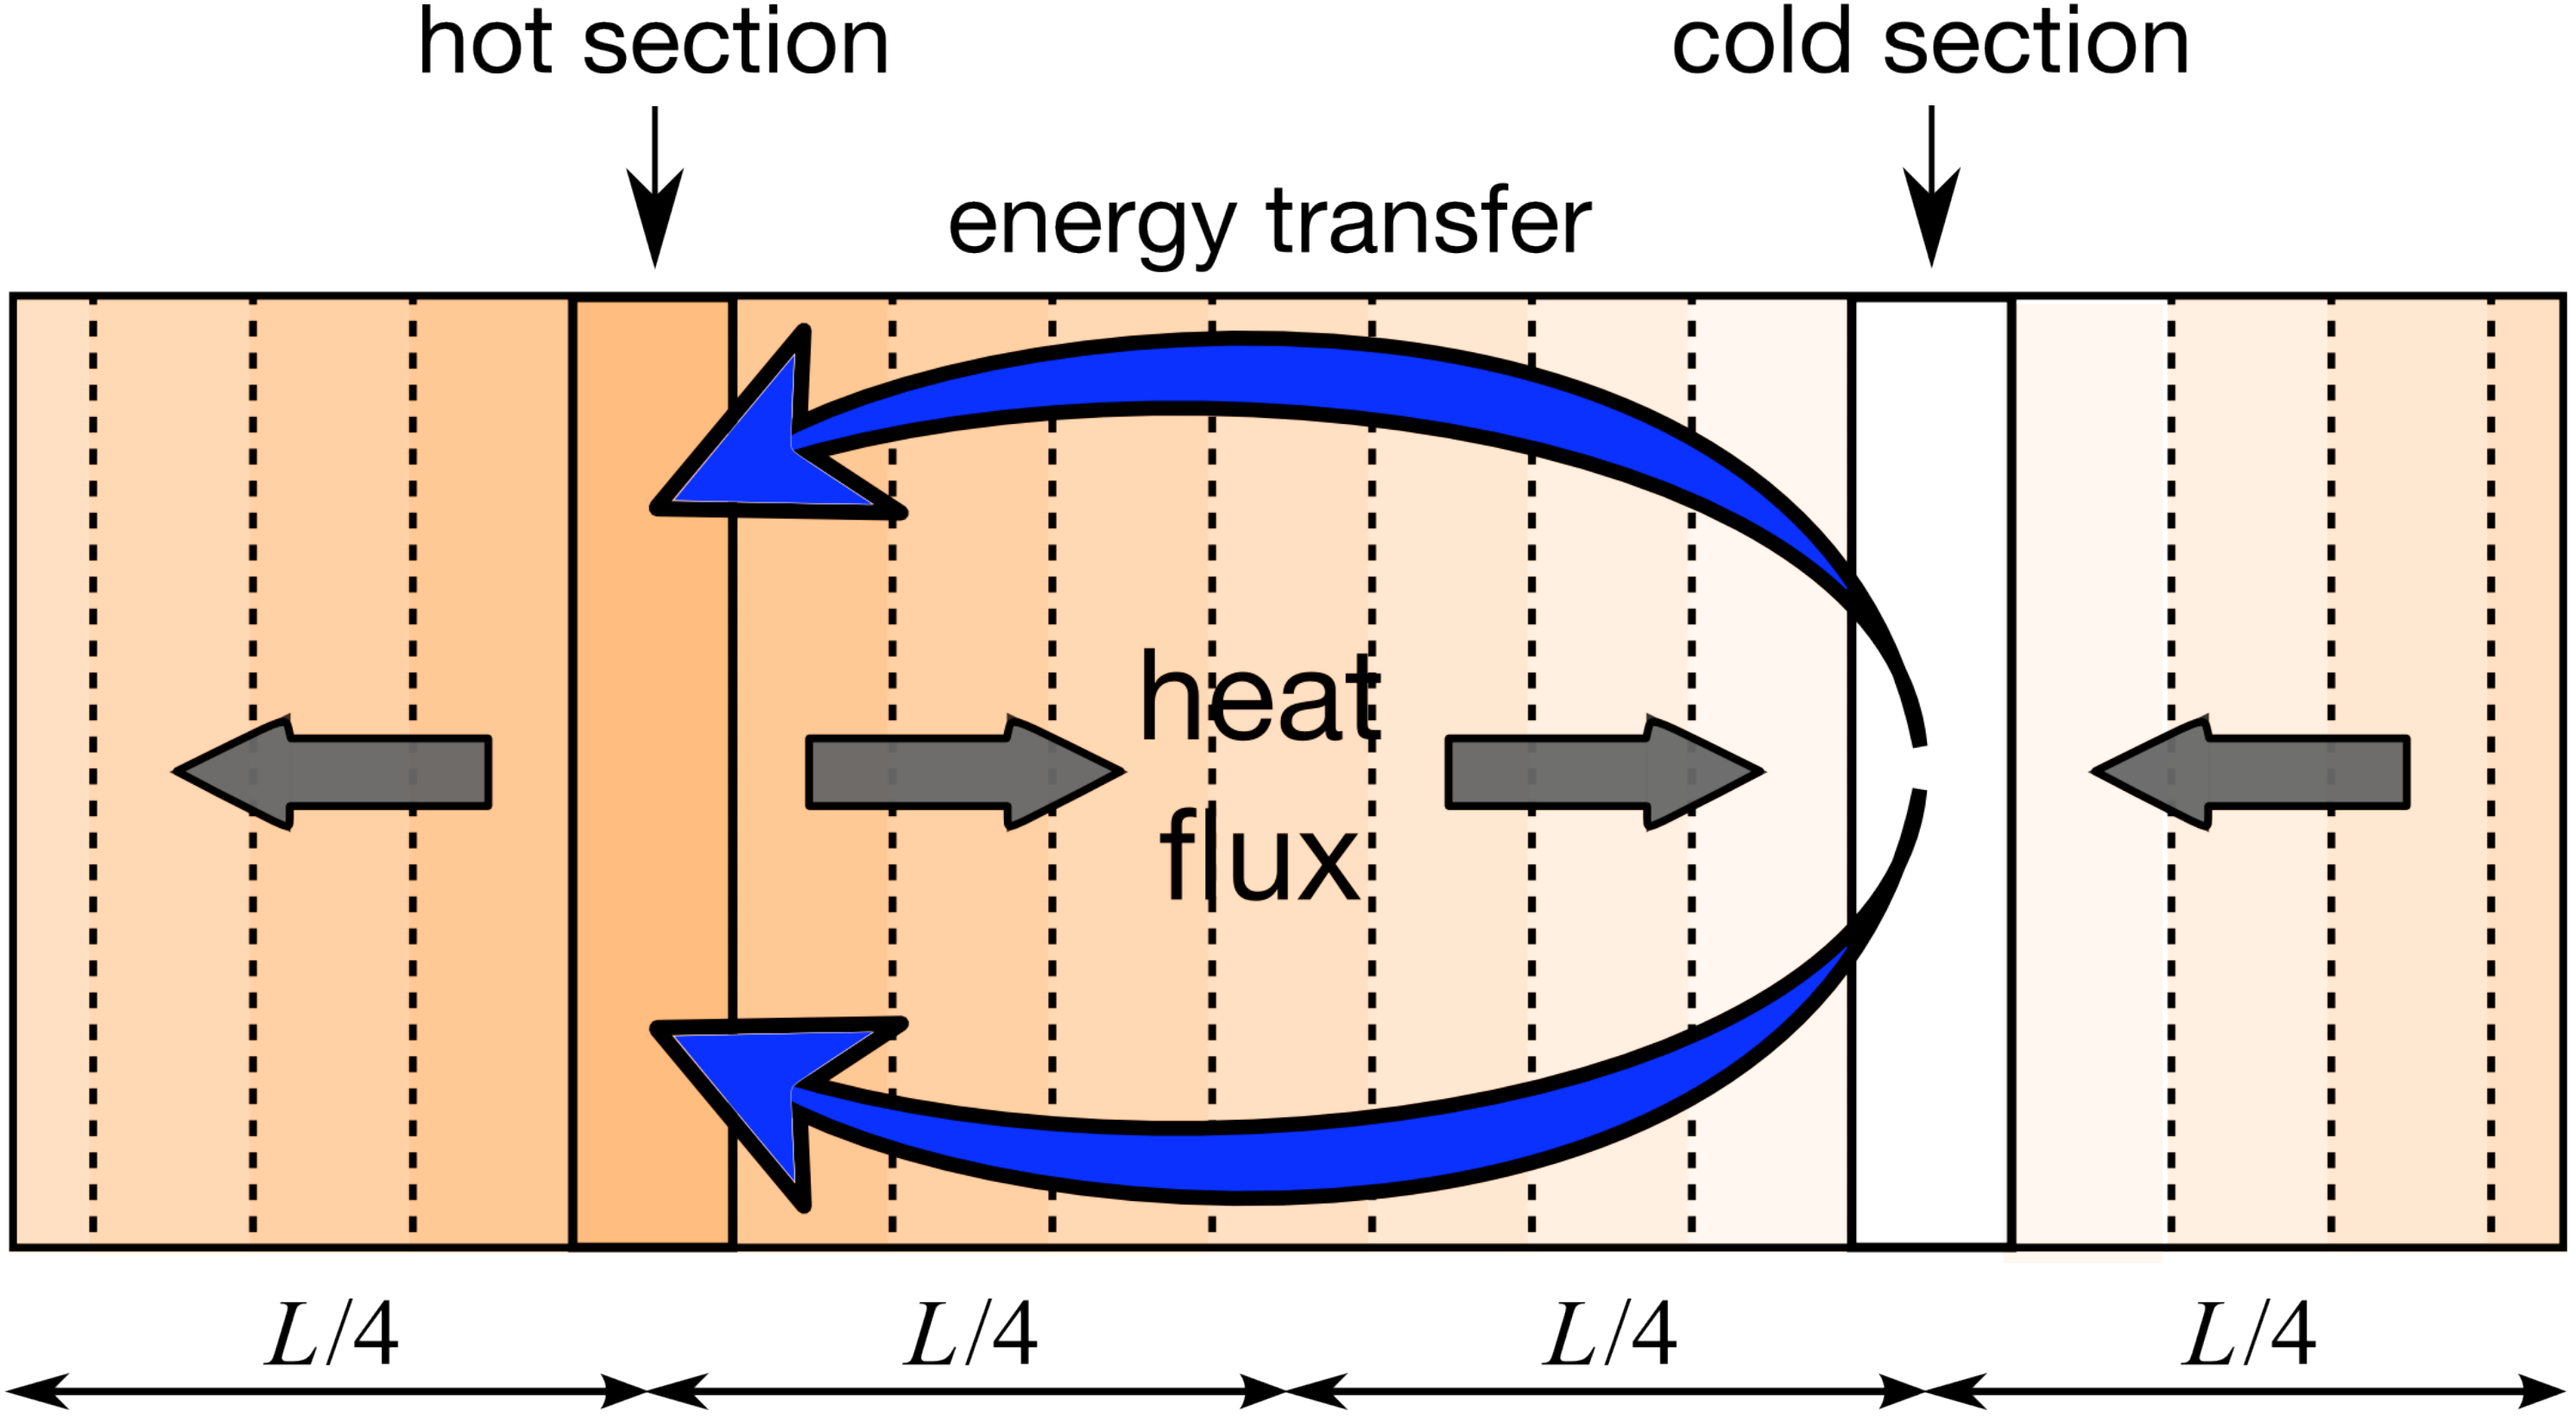
\includegraphics[width=\linewidth]{Figures/ss_direct_mod.png}
  \caption{Movement and distribution of heat in the direct method. Orange to white scale represents temperature \citep[modified from][]{Stackhouse2015}.}
  \label{fig:ss_direct}
\end{figure}

From kinetic theory [[[REF?]]], conductivities computed by the direct method ($k_L$) are dependent on length of simulation cell,
\begin{equation}
k_{L} = \frac{1}{3} C_{V} v l_{L} \label{length-dep},
\end{equation}

where $C_v$ is the volumetric heat capacity, $v$ is the average phonon drift velocity, and $l_L$ is the phonon mean free path. 

%-------------------
\subsubsection{Data processing}
%-------------------

The finite size of the simulation cell truncates the mean free path, underestimating conductivity compared to that of the bulk material ($k_\infty$). Using results from simulations of varying cell length ($L$), conductivity is extrapolated to a length-independent value (where $b$ is a material dependent parameter),

\begin{equation}
{k_{L}}^{-1} = b L^{-1} + {k_{\infty}}^{-1} \label{linear-extrap}.
\end{equation}

Inverse conductivities from direct method simulations are plotted against corresponding inverse cell lengths. A straight line is fit to the data and extrapolated to the y-axis (at which the inverse cell length equals zero and real length equals infinity), where the intercept gives the inverse of the bulk material conductivity \citep{Schelling2002}.

\begin{figure}[h]
  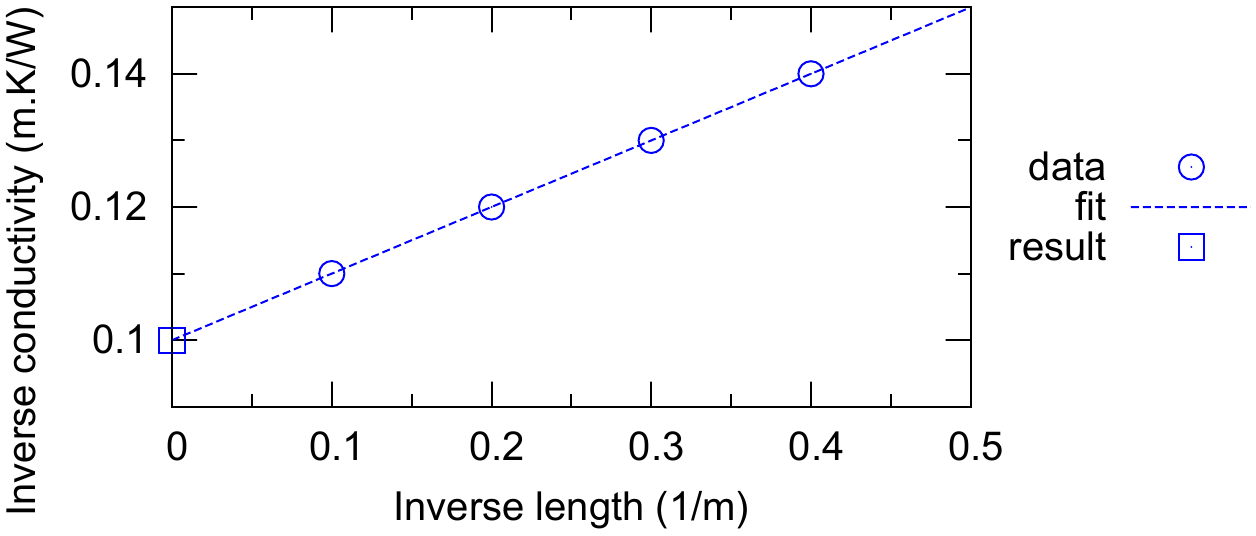
\includegraphics[width=\linewidth]{Figures/ideal_extrap.png}
  \caption{Idealised example of linear extrapolation procedure. Inverse computed conductivities are plotted against inverse simulation lengths. Extrapolation to y-axis gives conductivity of an infinite system length, i.e. the bulk material.}
  \label{fig:ideal}
\end{figure}

%-------------------
\subsubsection{Finite-size effects}
%-------------------

Problems arise when the data do not support a linear trend. There are two effects of finite system size that can cause an individual direct method simulation to diverge away from an inferred/expected linear trend, both of which result in overestimation of the length-dependent conductivity data point. First, when the distance between hot and cold sections (controlled by cell length) is shorter than the MFP, phonons travel ballistically (i.e. without any scattering events) from heat source to sink \citep{Sellan2010}. Conductivites in shorter length cells are overestimated when this occurs, reducing the gradient of the linear fit and thus underestimating the extrapolated conductivity.

For a given length, conductivity is dependent on the CSA, or aspect ratio of the simulation cell. Conductivity is overestimated due to an underestimation of phonon-phonon scattering, from sparse phonon phase sampling in cells where cross-section is small compared to length. Phonons that aren't resolved cannot contribute to phonon-phonon scattering effects. Reduced scattering means heat transport is artificially more efficient than expected from the bulk material. 

[[[SPECIFIC ALERT, REFERENCING THINGS I FOUND]]] However, the required CSA to abate this FSE is length-dependent. When the CSA is smaller than required for all cell lengths (e.g. 1x1 [FIGURE]), all conductivities are overestimated \citep[][albeit for nanotube diameter?]{Thomas2010}. As the CSA is increased, the data points (and thus also the extrapolated result) shift to lower conductivities (higher inverse conductivities). It is at this point that the short cells with lengths of similar order, will report conductivities converged with respect to CSA. Assuming these cells are sufficiently long to avoid the ballistic phonon transport (BPT), a linear fit can be extrapolated to obtain conductivity (for CSA around 2x2, the case at 4000~K). 

The convergence is not necessarily observed concurrently for longer cells however, where they may show overestimated conductivities compared to the fit through short cells (\cite{Hu2011}). This would cause the fit to all data to be steeper than it should, increasing the extrapolated result.  [[[HOPEFULLY THIS IS TRUE]]] I can show that increasing CSA does not change the computed conductivity at short lengths, but does reduce values from longer cells and bring them into alignment with the expected fit.

%I MOVED THIS DOWN HERE RECENTLY - DO NOT IGNORE %Considering systems of varying size, length-dependent conductivities are obtained from the direct method and extrapolated to the bulk material (\citet{Schelling2002}). The validity of this extrapolation procedure have been called into question (e.g. \citet{Sellan2010}), when a linear trend cannot be fit through the length-dependent conductivities. We describe finite-size effects (FSE) which cause the conductivity result of a simulation to diverge from the value expected by a linear trend, and offer a comparison with results obtained from the Green-Kubo method. The two methods have previously been compared (e.g. \citet{Schelling2002}, and have been found to give results in good agreement.

%By comparing results with the Green-Kubo method, we will constrain the cell lengths in the linear extrapolation region to mitigate these effects. 











%%%MOVE TO 3

%[[[SPECIFIC ALERT, REFERENCING THINGS I FOUND]]] The effect of FSE on conductivity results depends on the magnitude of conductivity/phonon MFP/physical conditions. At low kappa/low MFP/high T/ (my 4000~K), no BPT is observed, and short cells (>16 unit cells) can be used for extrapolation. In fact, short cells must be used to extrapolate, unless CSA considersations are made to ensure convergence of long cell results.
%[[[SPECIFIC ALERT, REFERENCING THINGS I FOUND]]] At high kappa/high MFP/low T (my 1000~K), BPT must considered at the shorter cells (just 6?). Effectively there is a "sweet-spot", a window of cell lengths for a given CSA that produce consistently-converged results. Long cells outside of the window require a larger CSA, short cells outside show BPT. At 4000~K the lower limit of the window is smaller than the minimum cell length considered, and the upper limit is between 16-24 unit cells. For 1000~K the lower limit of the window moves inside the simulated cell length range around 6-8 unit cells (OR MORE?). The upper limit of the window appears to be larger than 96 unit cells, including all long cells up to this value produces an extrapolation in agreement with GK.
%We have investigated this effect by varying CSA for a range of cell lengths, extrapolated conductivity decreases and eventually converges with CSA. We will use the smallest area that produces the converged conductivity for computational efficiency. 











%---------------------------------------
\subsection{Green-Kubo}
%---------------------------------------
The Green-Kubo method uses auto-correlation functions (ACFs) to quantify time-dependence of heat fluxes (shown in Figure~\ref{fig:gk_acf}, and Equation \ref{acf-j}), in a simulation cell of roughly cubic dimensions (WHY??) and spatially-consistent average temperature. Instantaneous heat fluxes can be used to determine how energy is dissipated within a system, where brief flux events mean heat is transferred quickly indicating high thermal conductivity [[[and vice versa, BUT IS THIS TRUE?]]]. 

\begin{figure}[h]
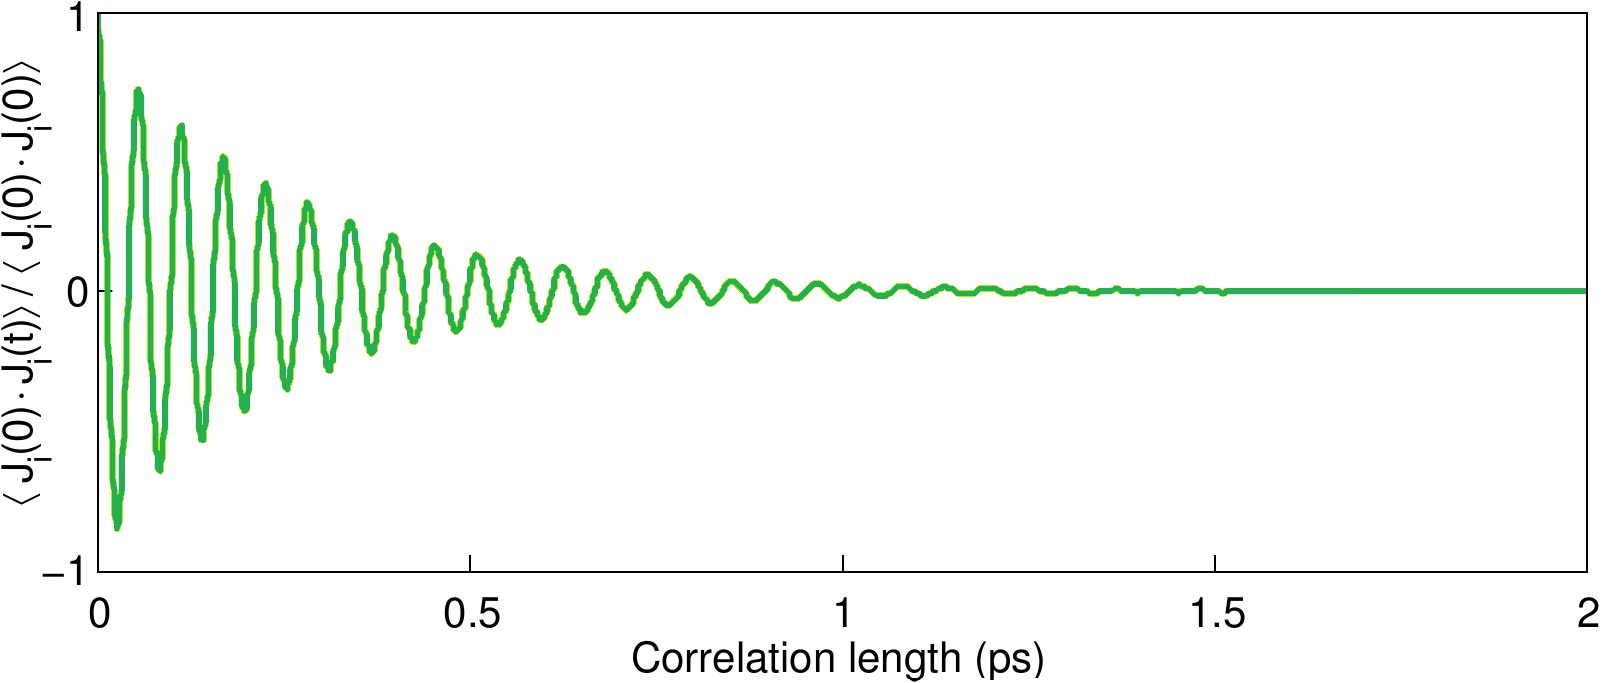
\includegraphics[width=\linewidth]{Figures/gk_acf.png}
\caption{Normalised ACF. Correlation is taken over a longer length than shown on this plot (100 ps), however the function decays to less than 1\% of its initial value at 2~ps. It continues to oscillate about zero, with a positive average value.}
\label{fig:gk_acf}
\end{figure}

The auto-correlation is obtained over the net heat flux series in each crystallographic direction, for a timescale up to a chosen correlation length.
~
\begin{equation}
ACF_i = \left \langle J_i(0) \cdot  J_i(t) \right \rangle,
\label{acf-j}
\end{equation}
~
where $i$ specifies direction, $J$ is heat flux, and $t$ is the correlation length. The integral of heat flux ACF is proportional to thermal conductivity via the Green-Kubo equation (see Figure~\ref{fig:gk_int} and Equation \ref{gk-int}), 
~
\begin{equation}
\kappa_i = \frac{V}{k_{B}T^{2}} \int_{0}^{\infty} \left \langle J_i(0) \cdot  J_i(t) \right \rangle dt ,
\label{gk-int}
\end{equation}
~
[[[I am using ``k''s and ``kappa''s to represent \tc, kappa here and k earlier?]]] where $V$ is the simulation cell volume, $k_B$ is the Boltzmann constant, and $T$ is the average temperature of the system. In this study we use Green-Kubo results as an independent check on the direct method, as they do not have the same finite size-effects. Obtaining a converged conductivity result simply depends on using a large enough cell volume / number of atoms. 

\begin{figure}[h]
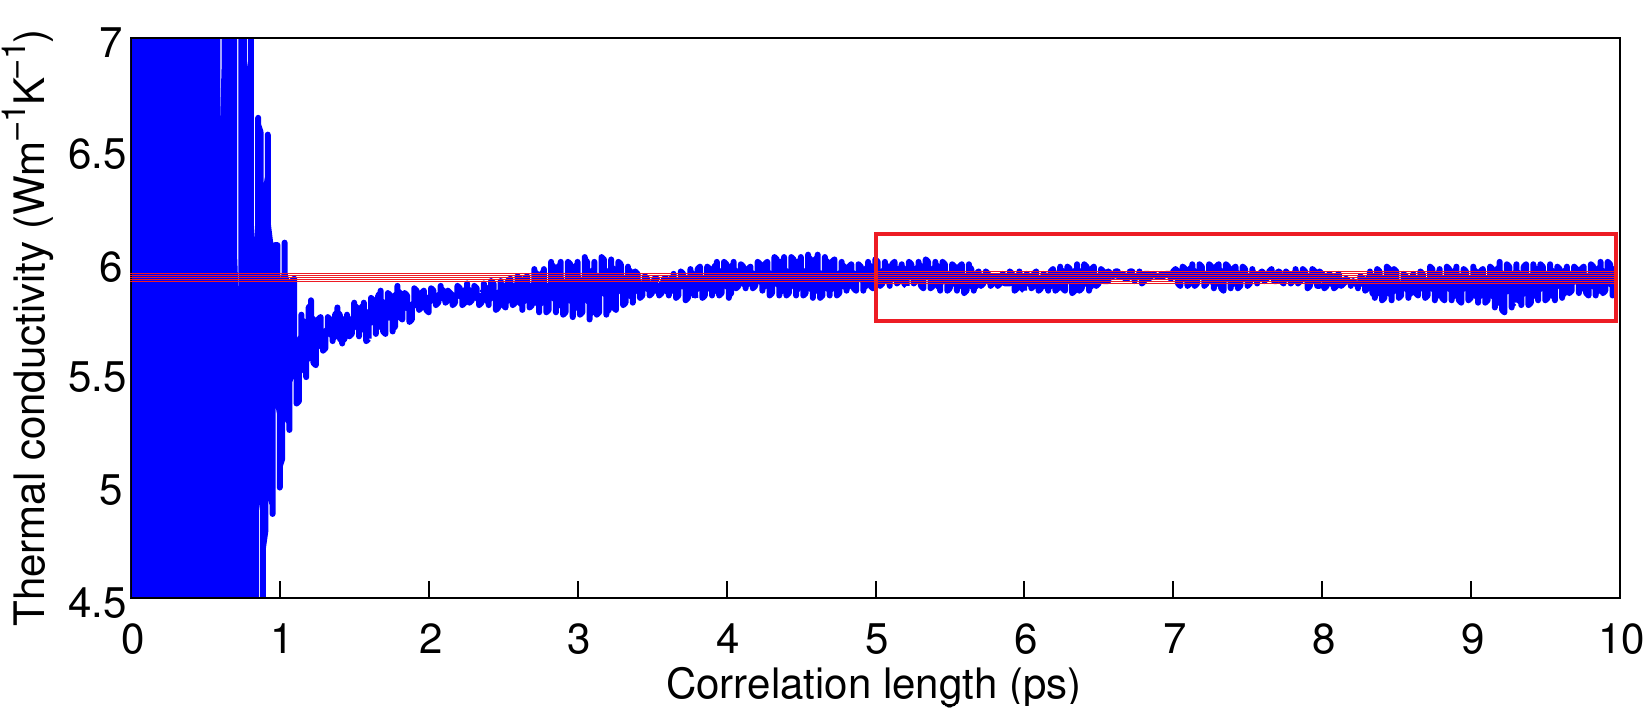
\includegraphics[width=\linewidth]{Figures/gk_int.png}
\caption{Integrated ACF, multiplied by constants to get thermal conductivity. Large variation in the first 1 ps corresponds to the correlation time where the ACF is unconverged (still decaying / large oscillations). Thermal conductivity is averaged from correlation time of 5~ps - 10~ps (region in red box).}
\label{fig:gk_int}
\end{figure}

The individual integrals obtained from the Green-Kubo show variation from the average combined integral on the order of the mean. Many simulations from different intital temperature conditions are required in order to ensure good sampling of conductivity, as well as ensuring the computation time for each is long enough for convergence. This makes Green-Kubo a computationally expensive method, especially for large systems.

The ACF should decay to zero as correlation time tends to infinity, however noise in the ACF prevents this. This will ultimately cause the integral to diverge/drift on long timescales. \citet{Howell2012} fits a series of exponential decays to their ACF, forcing the expected decay to zero and subsequent (constant) integral convergence. This is represents a significant improvement on the conductivity estimate at long correlation lengths, but is mostly similar with the un-fit integrals early in the correlation. (INTEGRAL DRIFT FIGURE, JUST THE ONE INTEGRAL FOR 100PS)

(STACKHOUSE 2010 REFERENCES Volz and Chen 2000; Sun and Murthy 2006)



%---------------------------------------
\subsection{Other}
%---------------------------------------
(3) Anharmonic lattice dynamics \citep{Tang2009}. %(BTE)CHERNATYNSKIY and PHILLPOT 2010?
\\
(4) Combined quasiharmonic lattice dynamics and molecular dynamics method \citep{DeKoker2009}.



%-----------------------------------------------------------
\section{Previous work}
%-----------------------------------------------------------

%---------------------------------------
\subsection{Method comparison}
%---------------------------------------

%---------------------------------------
\subsection{Finite-size effects}
%---------------------------------------
Should this section be interspersed into when FSE are mentioned in methods?

%-------------------
\subsubsection{STUFF THAT MIGHT BE WRONG BECAUSE FSE?}
%-------------------










%%-------------------
%\subsubsection{Parameter drift/convergence}
%%-------------------
%We ensure all calculations are run for a sufficient length of time for the conductivity value to converge. When conductivity fails to converge it means either the simulations needs to be run for longer (unlikely with our nanosecond-scale classical calculations), or the system temperature has drifted. When NVE simulations are run for a long time there is noticable drift in the average system temperature (due to numerical approximations in the equation of motion), which in turn causes drift in the computed conductivity.

%NPT-NVT-NVE PROCESS



 
% Chapter Template

\chapter{The Chapter formerly known as Paper 1} % Main chapter title

\label{Chapter3} % Change X to a consecutive number; for referencing this chapter elsewhere, use \ref{ChapterX}

\section{\label{sec:intro}Introduction}

\subsection{\label{sec:intro.intro}Intro Intro (remove this subsection header later)}
Knowledge of the thermal conductivity of solids is key in a wide range of technological applications and for our understanding of natural systems. For example, in the Earth's lower mantle thermal conductivity controls the nature of planetary convection (\citet{Tosi2013}), and the heat flux out of the core which powers the geotherm. Low thermal conductivities are required in thermoelectric materials, to maximise the efficiency of heat-electricity conversion (\citet{Snyder2008}).

A range of atomic scale simulation methods are available to determine the lattice thermal conductivity of materials. These are invaluable for calculating thermal conductivity at conditions of which experiments are difficult, e.g. the extreme conditions found in the Earth's lower mantle (pressures and temperatures up to 136~GPa and 4000~K at the core-mantle boundary).

(MOVE - to where though?) Many studies assume lowermost mantle thermal conductivity to be 10~\wmk~(e.g. \citet{Lay2008}), but uncertainty in the extrapolation of results made at low pressures and temperatures gives a range of 4~-~16 \wmk~(\citet{Brown1986, Osako1991, Hofmeister1999, Goncharov2009, Manthilake2011, Ohta2012}).
\chapter{Modelling the thermal conductivity of Fe-bearing bridgmanite at the CMB} % Main chapter title
%(Mg,Fe)SiO$_3$

\label{Chapter4} % Change X to a consecutive number; for referencing this chapter elsewhere, use \ref{ChapterX}

As stated earlier (REF), there are no are experiments that can reach the high pressures and temperatures necessary to replicate the conditions of the lower mantle. The addition of impurities into minerals further complicates the matter. In addition to pressure and temperature-dependence, composition must be considered for full evaluation.

DISCUSS/RE-ITERATE EARLIER-DISCUSSED SEMI-RELEVANT EXPERIMENTS HERE, MANTHILAKE

%-----------------------------------------------------------
\section{Simulating the effect of atomic impurities}
%-----------------------------------------------------------

The bulk of the lower mantle comprises bridgmanite (X\%, and its high-pressure polymorph post-perovskite), ferropericlase (Y\%), along with others (Z\%) such as calcium silicate perovskite CaSiO$_3$. The composition can vary within these mineral archetypes, significantly the concentration of iron impurities. Magnesium is replaced with iron in 
\mgsios and MgO compositions, leading to \fesios and FeO endmembers. Aluminium can similarly be subsituted for Magnesium (((REF))) (Mg$^{2+}$ + Si$^{4+}$ = Al$^{3+}$ + Al$^{3+}$ or Al$^{3+}$ + Fe$^{3+}$).
BRODHOLT NATURE PAPER

Impurities reduce \tcs by providing more opportunities for phonon scattering events. An impurity is an irregularity to a propagating phonon, much like a speedbumb to a car. They have different properties to the atoms the phonon expects to meet from crystal regularity, namely mass and their bonds with neighbouring atoms. For this reason that the \tcs of a solid solution is lower at intermediate compositions than at the endmembers. Even if one endmember has lower \cs than the other, an irregular mix of the two can produce even lower values.



%---------------------------------------
\subsection{How do impurities affect conductivity?} 
%---------------------------------------
\label{impur_theory}

The effect of impurities on lattice thermal conductivity is approximated by \citet{Klemens1960} and \citet{Padture1997}, a review of which can be found in the Supplementary Material of \citet{Stackhouse2015}. The lattice thermal conductivity of a binary solid solution is given \citep[in][Eq. S6]{Stackhouse2015} as
%
\begin{equation}
k_{\mathrm{S}}=k_{\mathrm{V}}\left ( \frac{\omega_{\mathrm{S}}}{\omega_{\mathrm{D}}} \right )\arctan \left ( \frac{\omega_{\mathrm{D}}}{\omega_{\mathrm{S}}} \right ),
\label{eq.SS2015SM.6}
\end{equation}
%
where $\omega_{\mathrm{S}}$ is the phonon frequency at which the mean free path is equal to that of the solute atoms, and $\omega_{\mathrm{D}}$ is the phonon frequency corresponding to the maximum of the acoustic branch in the phonon spectrum (the Debye frequency). $k_{\mathrm{V}}$ is the compositionally-weighted average of endmember conductivities, 
%
\begin{equation}
k_{\mathrm{V}}=\left ( 1-x \right )k_{1} + x\ k_{2} \ ,
\label{eq.SS2015SM.7}
\end{equation}
%
where $k_{\mathrm{1}}$ and $k_{\mathrm{2}}$ are the pure endmember conductivities, and $x$ is the decimal concentration of the second endmember \citep[][Eq. S7]{Stackhouse2015}.

Considering Eq. \ref{eq.SS2015SM.6}, when $\omega_{\mathrm{S}} \gg \omega_{\mathrm{D}}$, $\arctan(\omega_{\mathrm{D}}/\omega_{\mathrm{S}}) \rightarrow (\omega_{\mathrm{D}}/\omega_{\mathrm{S}})$, so $k_{S} \rightarrow k_{V}$, the conductivity considering impurities tends toward the endmember linear average. This will happen when other factors, such as high temperatures, have reduced conductivity and adding impurities has little additional effect.

On the other hand, when $\omega_{\mathrm{D}}\gg\omega_{\mathrm{S}}$, $\arctan(\omega_{\mathrm{D}}/\omega_{\mathrm{S}})\rightarrow\pi/2$, but $(\omega_{\mathrm{S}}/\omega_{\mathrm{D}})\ll 2/\pi$, so $k_{\mathrm{S}} < k_{\mathrm{V}}$, and impurity scattering has an effect on the resultant conductivity. Adding impurities has an effect like this when the conductivity has not already been reduced for other reasons, like at low temperatures compared to the conditions mentioned above. 

That factors which affect the severity of impurity scattering are temperature, the mass difference between the impurity and what it replaced, and the concentration of said replacements. The ratio of the phonon frequencies in Eq. \ref{eq.SS2015SM.6} can be expressed \citep[][Eq. S11]{Stackhouse2015} as
%
\begin{equation}
\left ( \frac{\omega_{S}}{\omega_{D}} \right )^{2} = \frac{1}{\left ( 6\pi^{2} \right )^{1/3}} \ \frac{T}{3 \varepsilon T_{S}} \ ,
\label{eq.SS2015SM.11}
\end{equation}
%
where $T$ is temperature, $T_{\mathrm{S}}$ is the temperature at which the phonon mean free path length approaches that of the interatomic seperation, and $\varepsilon$ is related to the mass difference and proportion of endmembers by
%
\begin{equation}
\varepsilon = \frac{\left (M_{2}-M_{1}  \right )^{2}}{\overline{M}^{2}} \ x\left ( 1-x \right ) \ ,
\label{eq.SS2015SM.9}
\end{equation}
%
where $M_{i}$ is the atomic mass of the $i$-th endmember, $\overline{M}$ is the mean atomic mass of the solid solution, and $x$ is the proporition of endmembers \citep[][Eq. S9]{Stackhouse2015}.

As the temperature increases, so too does the left-hand side of Equation \ref{eq.SS2015SM.11}. As discussed above, this reduces the effect of scattering caused by impurities, which will be relevant at CMB conditions. 

$\varepsilon$ increases with the mass difference of the endmembers, and the impurity concentration. Increasing $\varepsilon$ tends to reduce the phonon frequency ratio, meaning impurity scattering will affect the resultant conductivity more. The atomic masses of Mg and Fe are 24 and 56, so \fesios is 1.32 times heavier than \mgsio. As an aside, Equation~\ref{eq.SS2015SM.9} predicts that isotopic variations will have little effect on conductivity, where the mass changes are typically small (e.g. $^{24}$Mg to $^{25/26}$Mg) and abundances are low (Mg standard atomic weight is 24.3, the ratio of $^{24}$Mg to heavier isotopes is roughly 4:1).

The composition control term in Equation~\ref{eq.SS2015SM.9}, $x(1-x)$, increases from 0 to 0.25, when $x = 0.5$. $\varepsilon$ increases with composition up to 50\%, the furthest point away from both endmembers, therefore the condition of most disorder in the atomic structure.

!!! 181012 TALK ABOUT THESE EFFECTS AT CMB SPECIFICALLY and how they relate to the questions i'm posing?



%-----------------------------------------------------------
\section{Methodology}
%-----------------------------------------------------------

In this section I outline the process of taking Fe from chemistry to computer, by fitting my own coefficients to a Buckingham potential. I also go over how the Fe is incorporated into the \mgsio, considering its placement and concentration.

%---------------------------------------
\subsection{How does iron behave?} 
%---------------------------------------

I use two methods to introduce iron impurities to my bridgmanite models. The first approach is to simply create a magnesium atom with the mass of an iron atom, without changing any coefficients of the interatomic potentials from \citet{Oganov2000}. Despite being an obviously "quick and dirty" method, (I will show) this is a reasonable first-order approximation(((PROVE IT!?))). As the variation in mass number from Mg to Fe is large (24 to 56, a 133\% increase), it is likely to change the behaviour of the system more than a subtle change in the atomic interactions.

MENTION AMMANN IRON STUFF HERE

The second approach to add Fe into the \mgsios system is to fit interatomic potentials, as well as using the aforementioned mass change for a more realistic model. I adapted the \citet{Oganov2000} \mgsios Buckingham interatomic potential ($U$) to include the Fe-O interation. I determined two short-range potential parameters, $b$ and $\rho$, shown in Eq. 11 from \citet{Oganov2000},
%
\begin{equation}
U_{ij}\left ( R_{ij} \right ) = \frac{z_{i}z_{j}}{R_{ij}} + b_{ij}\ \textup{exp}\left ( - \frac{R_{ij}}{\rho_{ij}} \right ) - \frac{c_{ij}}{{R_{ij}}^{6}}, \label{og_buck}
\end{equation}
%
where $ij$ refers to an atom pair, $R$ is interatomic distance, $z$ is atomic charge, and $c$ relates to the Van der Waals force (zero for non O-O interactions). We determine $\rho$ in the same fashion as \citet{Oganov2000}, calculated from the atomic first ionisation potentials,
%
\begin{equation}
\rho_{ij} = \frac{1.85}{\sqrt{I_{i}}+\sqrt{I_{j}}}.  \label{urusov}
\end{equation}
%
$b$ is constrained using the GULP code \citep{Gale1997}, using the calculated $\rho$ value for Fe-O. We fit to the elasticity results of \citet{Parise1990}, an experimental study of (Mg$_{0.9}$,Fe$_{0.1}$)SiO$_3$ bridgmanite up to 433~K. Despite potential fitting being an improvement on solely changing mass (((PROVE IT!?))), it is still not perfect as the charge of our fitted Fe is not varied from the original Mg.

!!! Validate potentials

!!! Validate Fe vs. heavy Mg, isotope mass

!!! Include Oganov table (earlier?), with the fitted Fe info


%---------------------------------------
\subsection{Where do the impurities go?} 
%---------------------------------------

Iron is substituted with magnesium into the bridgmanite atomic structure. The unit cell contains 4~Mg atoms, and the smallest direct method cell I employ is a 6x2x2 supercell. Therefore the smallest amount of iron that can be added is 1/96 atoms, a concentration just over 1\%. A simple MATLAB script (((REF, APPENDIX))) is used to modify LAMMPS input files, randomly selecting a specified proportion of Mg atoms to be replaced with Fe. When a Mg atom changes to Fe, its mass and interatomic potential properties change. 

Due to the microscopic nature of the system, we do not want all of the added iron to be concentrated together in the simulation cell, especially in a heat source/sink region (((ELABORATE WITH FIGURE?))). To avoid this we order Mg atoms by length along supercell, and change a single atom every so many. For example, changing 1/4 atoms is different to changing 24/96. The latter has a higher variance in Fe per unit length, and the former chooses one atom to swap for every four along the system. After iron is added, the standard direct method or Green-Kubo workflow is followed.

!!! NICE PICTURE/DIAGRAM HERE?

!!! Comparison of random and homogeneous distribution, don't make reader engage their imagination, show obvious picture




%-----------------------------------------------------------
\section{Results}
%-----------------------------------------------------------

% reference SS2015 supp. for this section, the what affects conductivity bit
% have I gone too far into discussion here, interpretation of results?
Lattice thermal conductivities obtained from Green-Kubo calculations are plotted against temperature in Figure \ref{fig:kappa-temp_01}, for Mg and Fe-endmembers and the 50/50 solid solution mix.

Conductivity decreases with temperature, approximately following $\kappa \propto 1/T^{0.9}$ at the pressure of 136~GPa considered here. This is in contrast to the typically expected $\kappa \propto 1/T$ relation, indicating some kind of saturation in conductivity decrease with temperature.

\fesios has a consistently lower conductivity than \mgsio, which is to be expected due to the atomic mass increase [WRONG, SHEAR MOD DECREASE, DENSITY INCREASE, WAVESPEED EQUATION]. The two trends appear to be converging, indicating the conductivity of both species may be equal given a high enough (though unphysical for the lower mantle) temperature. This suggests there is a minimum conductivity associated with the crystal structure, reached first by \fesios with its inherently lower conductivity.

The 50\% solid solution has a consistently lower conductivity than \mgsio, and a lower than or equal to relation to \fesios. This is again to be expected, conductivity decreases from endmember to intermediate compositions as inpurity concentration increases. It can be seen that conductivity differences are very small at high temperatures for \fesios and the solid solution. If \fesios has already reached its theoretical minimum, adding impurities will do little to decrease it further.

\begin{figure}[h!]
  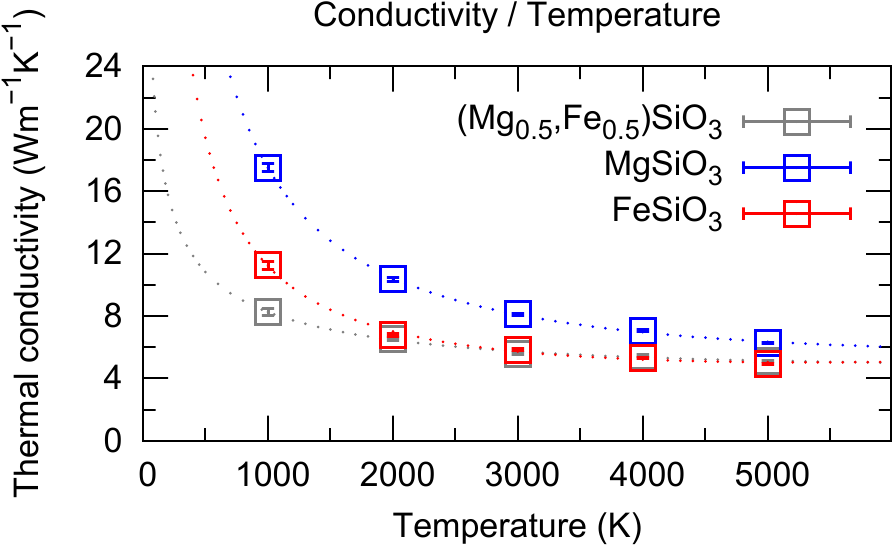
\includegraphics[width=\linewidth]{Figures/k-t_all_02.png}
  \caption{Data points are GK conductivity results, dotted line is the fit from Equation \ref{eq.okuda5_mod}.}
  \label{fig:kappa-temp_01}
\end{figure}

An alternative perspective to Figure \ref{fig:kappa-temp_01} is presented in Figure \ref{fig:kappa-comp_01}, where Green-Kubo conductivity results are plotted as a function of Fe impurity content for several temperature series.

Conductivity generally decreases with increasing temperature at all compositions, though the change becomes minimal at tempertatures above 3000~K.

The \mgsios endmember has a consistently higher conductivity than the \fesio. This can be explained by the general reduction in shear modulus and increase in density associated with adding Fe, which decreases seismic velocity and thus conductivity [TRUTH ALERT, REF???].

The amount of Mg atoms replaced with Fe has a variable effect on conductivity. A better way to label the effect is impurities added to an endmember, i.e. Fe is added to \mgsios and Mg to \fesio, which always serves increase phonon scattering and decrease conductivity. The decrease from this effect saturates towards a 50\% compositional mix. At high temperatures, this effect is minimal when adding Mg to \fesio. The conductivity could already be close to its theoretical minimum due to temperature effects, little reduction is observed from adding impurities.

\begin{figure}[h!]
  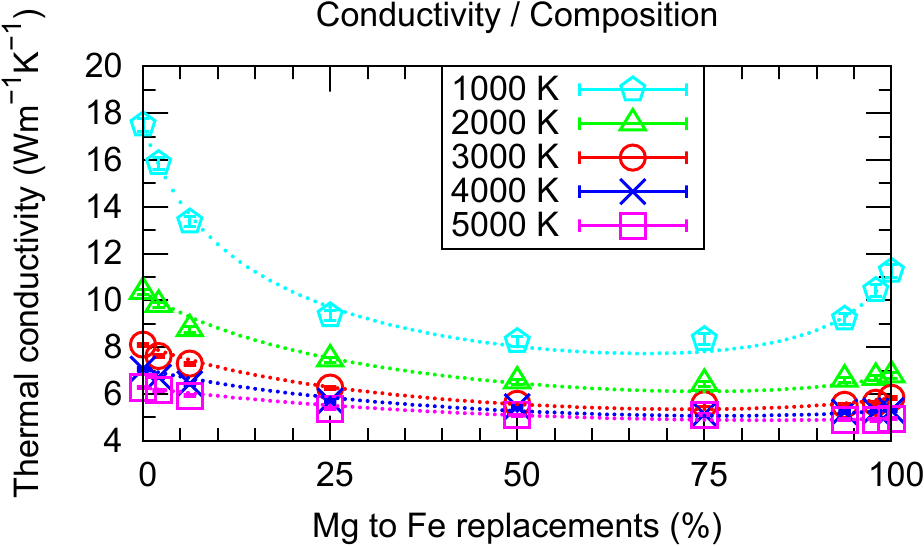
\includegraphics[width=\linewidth]{Figures/k-c_all_01.png}
  \caption{CAPTION}
  \label{fig:kappa-comp_01}
\end{figure}

A simple interpolation between endmember conductivities is insufficient, the presence of a compositional mix has an effect. This effect is itself temperature-dependent, the trough-like trend flattens with increasing temperature. These temperature and compositional dependences can be combined, allowing conductivity to be determined for a range of possible CMB conditions (Figure \ref{fig:kappa-temp-comp_01}). 

\begin{figure}[h!]
  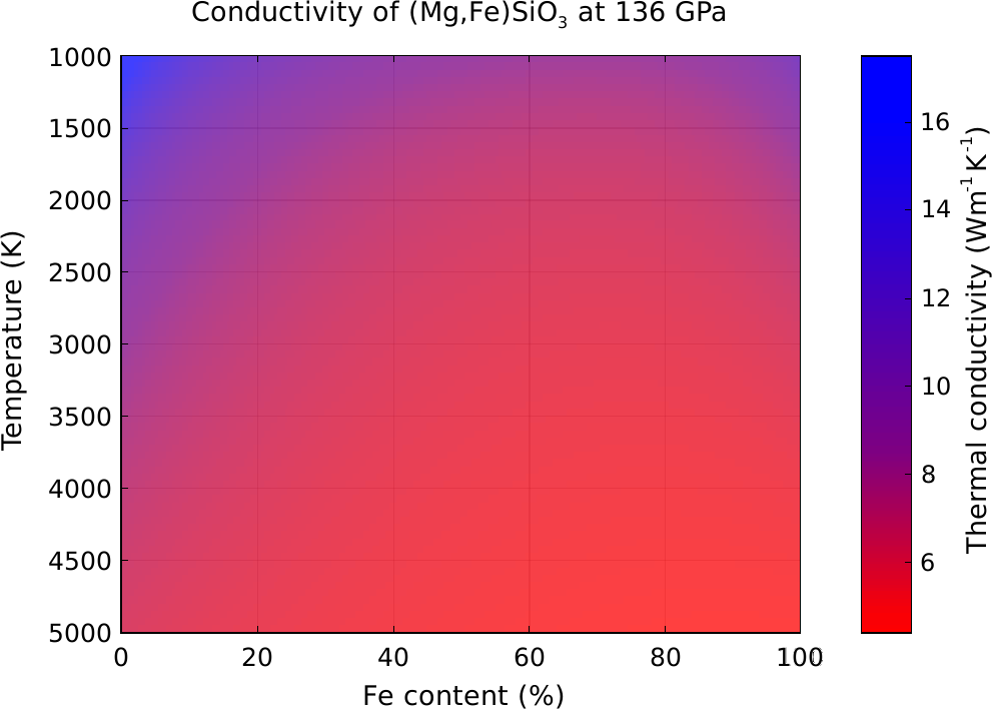
\includegraphics[width=\linewidth]{Figures/K_over_T_over_X.png}
  \caption{Modelled conductivity, shown plotted against temperature and composition. Note the sensitivity of the colour scale, showing low conductivities as dominant at high temperatures and intermediate compositions. High values are found only at low temperatures, and even then they rapidly decay and saturate to <8\wmk. Such conditions are unphysical at 136~GPa within the lower mantle.}
  \label{fig:kappa-temp-comp_01}
\end{figure}



%-----------------------------------------------------------
\section{Making the mantle model}
%-----------------------------------------------------------

In this section I develop a model for the lattice thermal conductivity of \mgfesios perovskite at CMB conditions. Whilst the CMB is a small section of the lower mantle, it marks the heat flow boundary from core to mantle, making it a very important region for studies of both sides of the interface. The pressure is 136~GPa, but I am interested in how temperature and Fe-content affect bridgmanite \tc.

Due to uncertainty in the lower mantle's composition, properties like \tcs are averaged considering the abundance of each mineral component. There are also solid solutions to consider however, particularly the concentration of Fe in \mgsio, as well as the phase boundary between bridgmanite and \mgsios post-perovskite. 

The conductivity of an intermediate composition is not a simple weighted average of the endmember values, you cannot interpolate linearly. This can be seen in Figure \ref{fig:kappa-temp_01}, where the (Mg$_{0.5}$,Fe$_{0.5}$)SiO$_3$ results do not plot between those of \mgsios and \fesio.



%%%%%%%%%%%%%%%%%%%%%%%%%%%%%%

%---------------------------------------
\subsection{Parameterising the data fit} 
%---------------------------------------

[Equations from \cite{Ohta2017} (eq. 7,8,9), and \cite{Okuda2017} (eq. 5)]

Equations and functional forms exist for the temperature and compostional dependence of \tc, and it is possible to combine the two. The basic idea is to determine the conductivity of \mgsios and \fesios endmembers at the temperature of interest, and then apply the (temperature-dependent) effect of composition.

\citet{Padture1997} propose a model for how impurities affect lattice thermal conductivity of a solid soultion, which \citet{Ohta2017}use to fit experimental ferropericlase data. Following a similar methodology, I fit the functional form to my (Mg,Fe)SiO$_3$ perovskite results at various temperatures (1000~K, 2000~K, 3000~K, 4000~K, and 5000~K). In an additional step, I establish the temperature-dependence of the fit constants. This means I am able to quantify the effect of composition at all temperatures.

\citet{Okuda2017} present a temperature scaling relation for lattice conductivity \citep[originally from][]{Manthilake2011}, fit to their experimental results of bridgmanite. I apply this temperature scaling to computational results of \mgsios and \fesios at 136~GPa. With the temperature dependence of these endmembers and of the compositional effect, I am able to able to determine the conductivity of any composition, at any temperature in the range 1000~K to 5000~K, at 136~GPa representative of the CMB.

The aforementioned temperature dependence from \citet{Manthilake2011} considers density, allowing conductivity to be determined as a function of temperature and pressure. In the examples I will present, I am only concerned with systems at 136~GPa. All density changes will result from thermal expansion, and the equations will be altered to accomodate this.

Some of the equations in the following section have already been presented as analogous forms in Section \ref{impur_theory}. The equations are kept similar to their published form, which was \citet{Stackhouse2015} in the former, and \citet{Ohta2017, Okuda2017} in the following.


    
%-------------------
\subsubsection{Compositional dependence}
%-------------------

\citet{Ohta2017} Eq.~7
\begin{equation}%-----
\kappa_{latt}=\kappa_{i}\left ( \frac{\omega_{0}}{\omega_{M}} \right )\mathrm{arctan}\left ( \frac{\omega_{M}}{\omega_{0}} \right )
\label{eq.ohta7}
\end{equation}%-------
\\ $\kappa_{latt}$ - output conductivity as function of t \& x (\wmk), considering mineral specific parameters\\
$\kappa_{i}$ - the composition-dependent conducitivity, if it were linearly interpolated between endmembers (\wmk)\\
$\omega_{0}$ - \enquote{\textit{the phonon frequency where the intrinsic mean free path is equal to that due to solute atoms (or just interatomic spacing?)}}\\
$\omega_{M}$ - \enquote{\textit{the phonon frequency corresponding to the maximum of the acoustic branch of the phonon spectrum (Debye frequency)}}\\

The two components $\kappa_{i}$ and $\omega_{0}/\omega_{M}$, are both temperature and composition-dependent. $\kappa_{i}$ gives the compositionally-weighted average conductivity, a linear interpolation between endmembers at a certain temperature. $\omega_{0}/\omega_{M}$ controls the conductivity decrease due to the impurity effect, the magnitude of which depends on the temperature and composition of interest.

By combining models for the temperate-dependence of \mgsios and \fesio-endmember conductivities, and the fit $\chi^{T}$ parameter, I obtain a function for conductivity of the lower mantle (136~GPa) as a function of just temperature and composition (as illustrated in Figure. \ref{fig:kappa-comp_01}).\\




Ohta eq. 8 
\begin{equation}%-----
\left ( \frac{\omega_{0}}{\omega_{M}} \right )^{2}=\frac{\chi^{T}}{C\left ( 1-C \right )}  
\label{eq.ohta8}
\end{equation}%-------
$\omega_{0}$ - \enquote{\textit{the phonon frequency where the intrinsic mean free path is equal to that due to solute atoms (or just interatomic spacing?)}}\\
$\omega_{M}$ - \enquote{\textit{the phonon frequency corresponding to the maximum of the acoustic branch of the phonon spectrum (Debye frequency)}}\\
$\chi^{T}$ -temperature-dependent parameter to \dots ??? \\
$\chi$ - \enquote{\textit{a constant}}\dots\\
$T$ - temperature of interest (K, default data fit between 1000 - 5000 K, but extrapolation should be reasonable)\\                    
$C$ - composition mix of interest (dimensionless, values between 0 and 1)\\

The equation splits $\omega_{0}/\omega_{M}$ into its temperature and composition-dependent components, where $\chi$ is a temperature-dependent variable. A value for $\chi$ is fit for all compositions at each temperature. $C\left ( 1-C \right )$ is largest when $C=0.5\ or\ 50\%$, relating to the shape of the trough formed by this fit.\\

$\chi^{T}$ scaling 
\begin{equation}%-----
\chi^{T}=A T^{B}
\label{eq.chi_scale}
\end{equation}%-------
\\ *$\chi^{T}$ -temperature-dependent parameter to \dots ??? \\
*$\chi$ - \enquote{\textit{a constant}}\dots\\
*$T$ - temperature of interest (K, default data fit between 1000 - 5000 K, but extrapolation should be reasonable)\\                    
$A$ - coefficient in $\chi^{T}$ variation with temperature\\
$B$ - exponent in $\chi^{T}$ variation with temperature\\

In order to obtain an equation for conductivity at any mantle temperature, it is required that $\chi$ can be expressed as function of temperature. Figure \ref{fig:draft_xt} shows $\chi$ over $T$ fit with a power law and 4th order polynomial, the former of which is a poor fit and the latter an egregious overfitting. 

\begin{figure}[h]
  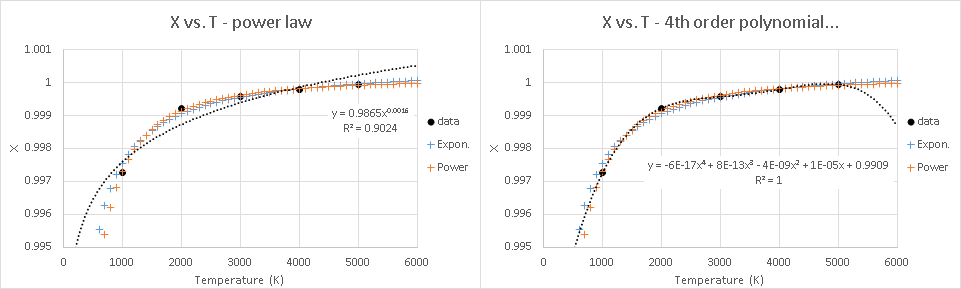
\includegraphics[width=\linewidth]{Figures/draft_XT.png}
  \caption{The fit $\chi$ values plotted against $T$, with power law (left) and 4th order polynomial (right) trendlines. Blue and orange series are the exponential and power law fits obtained from plotting $\chi^T/T$ (see Figure \ref{fig:draft_xtt}).}
  \label{fig:draft_xt}
\end{figure}

The lack of an obvious trend in $\chi$ against $T$ can be countered by plotting $\chi^T$ over $T$, and fitting either a expontial or power law relationship (Figure \ref{fig:draft_xtt}). I use the power law-relationship as it represents the temperature-dependence better, both statistically and sensitivity-wise. The value of $\chi^T$ at high $T$ has a lesser effect on the conductivity-composition relationship than at low $T$, where the power law fit matches the data closer. In Figure \ref{fig:draft_xt}, we can see that either of the power law or exponential $\chi^T/T$ fits represent the data better than the $\chi/T$ relations.\\ 

\begin{figure}[h]
  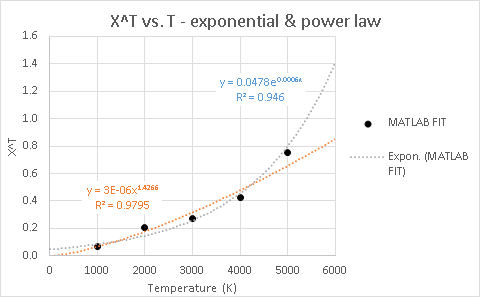
\includegraphics[width=\linewidth]{Figures/draft_XTT.png}
  \caption{Exponential fit in blue (more curved), power law in orange (flatter)}
  \label{fig:draft_xtt}
\end{figure}



Ohta eq. 9 
\begin{equation}%-----
\kappa_{i}=\left ( 1-C \right )\kappa_{\mathrm{MgSiO_{3}}}+C\ \kappa_{\mathrm{FeSiO_{3}}}
\label{eq.ohta9}
\end{equation}%-------         
\\ *$\kappa_{i}$ - the composition-dependent conducitivity, if it were linearly interpolated between endmembers (\wmk)\\
*$C$ - composition mix of interest (dimensionless, values between 0 and 1)\\
$\kappa_{MgSiO_{3}}$ - temperature and volume-dependent conductivity for Mg endmember (\wmk)\\
$\kappa_{FeSiO_{3}}$ - temperature and volume-dependent conductivity for Fe endmember (\wmk)\\

This equation describes the conductivity of an intermediate composition, assuming the relation is a simple weighted mean. $C$, in this case specifically, is the proportion of Fe atoms swapped into the system for Mg. The actual dependence of conductivity with composition is more complicated, this intermediate average value is adjusted for atomic-scale effects in Equation.~\ref{eq.ohta7} \citep[][Eq. 7]{Ohta2017}. \\

%-------------------
\subsubsection{Temperature dependence}
%-------------------

\cite{Okuda2017}\\

Okuda eq. 5 

\begin{equation}%-----
\kappa_{adj}=\kappa_{\mathrm{ref}}\left ( \frac{\rho}{\rho_{\mathrm{ref}}} \right )^{g}\left ( \frac{T_{\mathrm{ref}}}{T} \right )^{a}
\label{eq.okuda5}
\end{equation}%-------
\\ $\kappa_{adj}$ - temperature and density-dependent conductivity of an endmember (\wmk)\\
$\kappa_{ref}$ - reference conducitivty\\
$T_{ref}$ - reference temperature\\
$a$ - exponent controlling temperature-dependent conducitvity of an endmember\\
$\rho_{ref}$ - reference density\\
$g$ - exponent controlling density-dependent conducitvity of an endmember\\

\citet{Okuda2017} use a model for density and temperature-dependent conductivity (((from Manthilake 2011, REF???))), which utilises exponents obtained from REAL data / is calculated? (actually real numbers, only mine are fitted?). A reference value is scaled to infer conductivity at the conditions of interest, which in this case is temperature and pressure (via proxy using simulation cell volume/density).\\



Okuda eq. 5 modified

\begin{equation}%-----
\kappa_{\mathrm{adj}}=\kappa_{\mathrm{ref}}\left ( \frac{T_{\mathrm{ref}}}{T} \right )^{a}\left ( \frac{V_{\mathrm{ref}}}{V} \right )^{g}
\label{eq.okuda5_mod}
\end{equation}%-------
\\ $T_{\mathrm{ref}}$ - temperature at which reference conductivity is calculated (K)\\
$T$ - temperature of interest to interpolate (K, default data fit between 1000 - 5000 K, but extrapolation should be reasonable)\\   
$V_{\mathrm{ref}}$ - reference volume of an endmember (E-30 m$^3$)\\
$V$ - temperature-dependent volume of an endmember (E-30 m$^3$)\\
$h$ - exponent controlling volume-dependent conducitvity of an endmember\\

I adapt Eq. \ref{eq.okuda5} to consider volume instead of density (Eq. \ref{eq.okuda5_mod}), where density and volume are inversely proportional. Varying $a$ and $h$ I fit this equation for both Mg and Fe endmembers, using reference values from 1000~K (see Figure \ref{fig:kappa_temp_01}). The purpose of this is to scale the conductivities needed for Eq. \ref{eq.ohta9} to any temperature of interest.





\pagebreak

The lattice thermal conductivity (in \wmk) of a material as a function of temperature and composition can be approximated by the following equation,
%
\begin{equation}
\kappa_{\mathrm{latt}}=\kappa_{\mathrm{i}}\left ( \frac{\omega_{\mathrm{0}}}{\omega_{\mathrm{M}}} \right )\mathrm{arctan}\left ( \frac{\omega_{\mathrm{M}}}{\omega_{\mathrm{0}}} \right ),
\label{eq.ohta7}
\end{equation}
%
where $\omega_{\mathrm{0}}$ is the phonon frequency at which the mean free path is equal to that of the solute atoms, and $\omega_{\mathrm{M}}$ is the phonon frequency corresponding to the maximum of the acoustic branch in the phonon spectrum (the Debye frequency). $\kappa_{\mathrm{i}}$ is the conductivity of the solid solution in the absence of impurity scattering, the linear interpolation to a composition between endmembers,
%
\begin{equation}
\kappa_{\mathrm{i}}=\left ( 1-C \right )\kappa_{\mathrm{MgSiO_{3}}}+C\ \kappa_{\mathrm{FeSiO_{3}}}\ ,
\label{eq.ohta9}
\end{equation}
%
$C$ being the decimal concentration of Fe impurities, with $\kappa_{\mathrm{MgSiO_{3}}}$ and $\kappa_{\mathrm{FeSiO_{3}}}$ as the temperature dependent conductivities of the endmembers. The ratio of the phonon frequencies can be expressed as
%
\begin{equation}
\left ( \frac{\omega_{\mathrm{0}}}{\omega_{\mathrm{M}}} \right )^{2}=\frac{\chi^{T}}{C\left ( 1-C \right )}\ ,
\label{eq.ohta8}
\end{equation}
%
where $\chi$ is a constant to be fit, and $T$ is the temperature of interest. $\chi$ can be thought as a measure of resistance to the effects of impurity scattering. For a given $T$ and $C$, increasing $\chi$ increases the phonon frequency ratio $\left ( \frac{\omega_{\mathrm{0}}}{\omega_{\mathrm{M}}}\right )$ which, as discussed in Section \ref{impur_theory}, means $\kappa_{\mathrm{latt}}$ tends towards $\kappa_{\mathrm{i}}$. $\chi$ is fit to the data at each temperature, but for the model we need it as a function of temperature. Figure \ref{fig:draft_xt} shows $\chi$ over $T$ fit with a power law (a.) and 4th order polynomial (b.), the former of which is a poor fit and the latter an egregious overfitting. 

\begin{figure}[h!]
  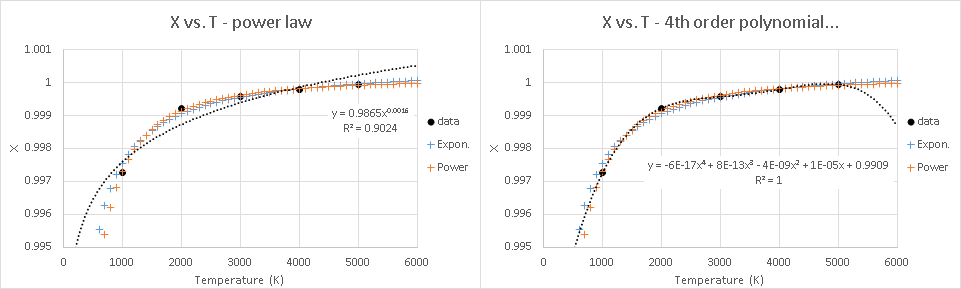
\includegraphics[width=\linewidth]{Figures/draft_XT.png}
  \caption{The fit $\chi$ values plotted against $T$, with power law (left) and 4th order polynomial (right) trendlines. Blue and orange series are the exponential and power law fits obtained from plotting $\chi^T/T$ (see Figure \ref{fig:draft_xtt}).}
  \label{fig:draft_xt}
\end{figure}

The lack of an obvious trend in $\chi$ against $T$ can be countered by plotting $\chi^T$ over $T$, and fitting either a expontial or power law relationship (Figure \ref{fig:draft_xtt}). I use the following power law-relationship, 
%
\begin{equation}%-----
\chi^{T}=A T^{B},
\label{eq.chi_scale}
\end{equation}%-------
%
where $A$ is the coefficient and $B$ is the exponent to be fit. This fit represents the temperature-dependence better, both statistically and sensitivity-wise compared to an exponential relationship $\left ( \chi^{T}=A e^{BT}\right )$. The value of $\chi^T$ at high $T$ has a lesser effect on the conductivity-composition relationship than at low $T$, where the power law fit matches the data closer. In Figure \ref{fig:draft_xt}, we can see that either of the power law or exponential $\chi^T/T$ fits represent the data better than the $\chi/T$ relations.

\begin{figure}[h]
  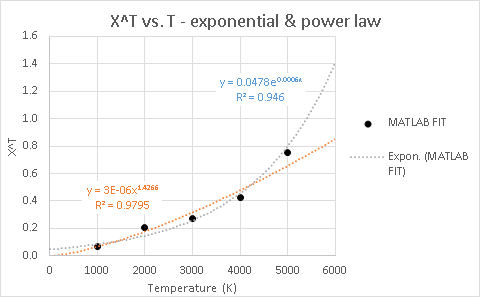
\includegraphics[width=\linewidth]{Figures/draft_XTT.png}
  \caption{Exponential fit in blue (more curved), power law in orange (flatter)}
  \label{fig:draft_xtt}
\end{figure}

The conductivities of $\kappa_{\mathrm{MgSiO_{3}}}$ and $\kappa_{\mathrm{FeSiO_{3}}}$ from Equation \ref{eq.ohta9} can be scaled with temperature, giving an adjusted value 
%
\begin{equation}
\kappa_{\mathrm{adj}}=\kappa_{\mathrm{ref}}\left ( \frac{\rho}{\rho_{\mathrm{ref}}} \right )^{g}\left ( \frac{T_{\mathrm{ref}}}{T} \right )^{a}.
\label{eq.okuda5}
\end{equation}
%
$\rho$ is density, $g$ and $a$ are exponents which control the nature of the density and temperature-dependence, and ``ref'' denotes a reference value. This equation is fit to the data, anchored around the values of the reference data point. I fit to the data point at 1000~K, as the conductivities at higher temperatures become more similar, converging towards a minimum point. Anchoring to 1000~K reduces the error in the fit, on account of the relatively larger conductivity at this temperature.

$$\frac{\rho }{\rho _{\mathrm{ref}}} \equiv \frac{V_{\mathrm{ref}}}{V}$$

$$\kappa_{\mathrm{adj}}=\kappa_{\mathrm{ref}}\left ( \frac{V_{\mathrm{ref}}}{V} \right )^{g}\left ( \frac{T_{\mathrm{ref}}}{T} \right )^{a}$$

$$g=\left( \partial \ln \kappa_{\mathrm{latt}} / \partial \ln \rho \right) _{T}$$

$$h \sim \left( \partial \ln \kappa_{\mathrm{latt}} / \partial \ln \rho \right) _{P}$$

$$\frac{V_{\mathrm{ref}}}{V(T)} \approx  mT+c$$

$$\kappa_{\mathrm{adj}}=\kappa_{\mathrm{ref}} \left ( mT+c \right )^{h} \left ( \frac{T_{\mathrm{ref}}}{T} \right )^{a}$$

















%Volume scaling ($y=mx+c$)  

%\begin{equation}%-----
%V=\frac{\partial V}{\partial T} T+V_{T_{0}}
%\label{eq.vol_scale}
%\end{equation}%-------     
%\\ *$V$ - temperature-dependent volume of an endmember (E-30 m$^3$)\\          
%${\partial V}/{\partial T}$ - fit gradient, change of volume with temperature (E-30 m$^3$/K)\\
%*$T$ - temperature of interest (K, default data fit between 1000 - 5000 K, but extrapolation should be reasonable)\\
%$V_{T_{0}}$ - intercept volume for T=0~K (E-30 m$^3$)\\

%I take Eq.~\ref{eq.okuda5} \citep[][Eq. 5]{Okuda2017} a step further, by obtaining $V$ in terms of $T$. This dependence is effectively linear over the temperatures considered (see Figure \ref{fig:draft_vt}). With this, Eq. \ref{eq.okuda_mod} can be made into a function of just temperature, meaning Eq.~\ref{eq.ohta7} \citep[][Eq. 7]{Ohta2017} is dependent solely on temperature, composition, and fit or calculated constants.

%\begin{figure}[h]
%  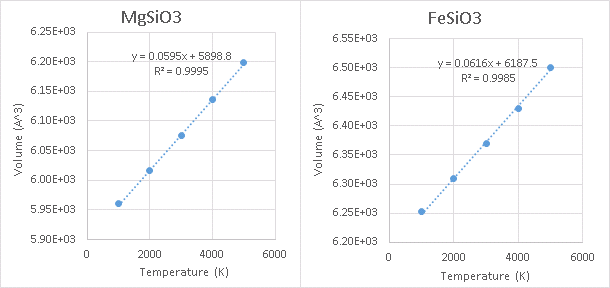
\includegraphics[width=\linewidth]{Figures/draft_VT.png}
%  \caption{Number of atoms is kept constant for all volumes, data is obtained from GK calculations of a 4x4x3 simulation cell. Magnitude of volume isn't of interest, just the relative difference to the reference volume.}
%  \label{fig:draft_vt}
%\end{figure}



\pagebreak


 
% Chapter Template

\chapter{Using STUFF to do THINGS} % Main chapter title

\label{Chapter5} % Change X to a consecutive number; for referencing this chapter elsewhere, use \ref{ChapterX}

%-----------------------------------------------------------
\section{Introduction}
%-----------------------------------------------------------

Many variables affect heat flux across core-mantle boundary (CMB). On the mantle side, they are the properties of the thermal boundary layer (TBL), the chemistry, temperature, and thickness. As explained in Chapter~\ref{Chapter4}, \tcs is dependent on the temperature and composition of a mineral. The thermal gradient away from the CMB depends on the thickness and temperature at the top and bottom of the TBL. Recalling Fourier's law once more, heat flux ($q$) is equal to the product of the thermal conductivity ($\kappa$), and the temperature gradient ($\nabla{T}$)
%
\begin{equation}
q=-\kappa \nabla{T}\ . 
\label{eq:fourier5}
\end{equation}

%---------------------------------------
\subsection{Approaching the problem}
%---------------------------------------

A simple one-dimensional model is not sufficient to describe the Earth, recalling Section~\ref{sec:LM}, two large low shear velocity provinces (LLSVPs) sit approximately on opposite sides of the CMB. A two-dimensional model, around the equator perhaps, would better describe the situation, but the CMB is spherical. A more sophisticated model is required to model changes in CMB structure with varying latitude and longitudes.

%---------------------------------------
\subsection{Introducing LEMA}
%---------------------------------------

!!! Need to introduce LEMA

Using LEMA, I specify a CMB base condition, and a TBL condition at some height above it. In all models I consider, the CMB will be isothermal. The TBL will have a variable mean temperature, and regions of higher and lower temperature. The lower mantle has an average Fe\%, but the LLSVPs are enriched compared the depleted surrounding bulk lower mantle. By varying the temperature and composition at the CMB, conductivity can be altered using the model from Section~\ref{sec:kappa_model}. The difference in temperature between CMB and TBL, and the undulations on the latter, control the lower mantle temperature gradient. 

The magnitude of the heat flux will change with parameters, perhaps more interesting is the lateral variation of this parameter. This will show how the lower mantle heat flux is sensitive to the conditions therein, and what condition or combination of conditions is most significant. The results from these calculations can then be compared to observables, dismissing scenarios which are unfeasible or unstable. There are many variables in the lower mantle, and observables to compare to. The variable conductivities from this work will play an important role in constraining CMB heat flux.

I can use spherical harmonics to generate structures that resemble LLSVPs. The centre of LLSVPs are approximately(/loosely?) located on the equator, antipodal at $0\degsym$ and $180\degsym$ longitude (the African and Pacific LLSVPs respectively). A first order approxiamtion for this geometry is the spherical harmonic $Y^{2}_{2}$, four quadrants of varying polarity around the polar axis. This looks good, but the projection is misleading in that it actually extends to the poles. It can be improved by stacking $Y^{0}_{2}$ on top of it, enhancing regions on the equator and reducing everything towards the poles. The results is two circular patterns, each located at opposite sides of the equator.

%$Y^{m}_{l}$

\begin{figure}[h]
  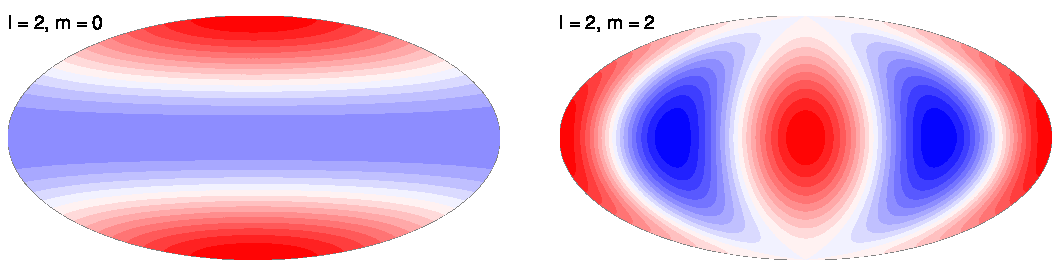
\includegraphics[width=\linewidth]{Figures/sph_harm.png}
  \caption[SPHERICAL HARMONICS]{Source: http://www-udc.ig.utexas.edu/external/becker/teaching-sh.html
  
These two harmonics are added together, amplifying blue regions on the equator, and diminshing everything else.}
  \label{fig:spherical_harmonics_diagram}
\end{figure}

For the $Y^{2}_{2}$ pattern, the areas of positive and negative amplitude regions are equal. For the  $Y^{0}_{2}$-combined model, the distribution of polarities is not even. By the way something like temperature is set up in the model, having a mean value with a ``$\pm$'' range leads to hotter hots, and warmer colds. There is more of the cold, surrounding mantle compared to LLSVP-designated regions, the LLSVPs have to be hotter than the surrounding mantle is colder.

Conductivity cannot be probed from the surface, but seismic velocities can be inferred from tomography. The same processes that affect conductivity generally affect shear wave velocity in the same fashion, be it increase or decrease. I can use $V_{\mathrm{S}}$ observations as an analogue to make inferences about the lower mantle.

When conductivity is kept constant across the whole CMB, variations in heat flux are determined solely by the lower mantle temperature profile. The reverse is also true, with constant temperature gradient above the CMB, conductivity controls lateral heat flow variations. This is a vast oversimplification, just talking about possible endmembers, in reality there will be both temperature and compositional factors affecting heat flux. Conductivity itself is temperature-dependent, further tying the two variables together.

When modelling LLSVPs, we are assuming they are thermochemical piles, that they are hotter and denser (e.g. high Fe\%) than the surrounding lower mantle. Increasing temperature reduces conductivity, as does increasing impurity inclusion. By modelling LLSVPs as purely thermal piles (i.e. increasing their temperature), we see a reduction in heat flux. This flux is further reduced when Fe content is increased, as conductivity decreases with impurity content. By altering temperature and composition in tandem, I will be able to suggest sets of lower mantle conditions which reproduce observations.

While this model is of dubious use in constraining the exact nature of CMB heat flux, inferences can be made on the relative variations laterally. How much heat is impeded passing through a LLSVP? How extreme do temperature and compositional variations need to be to significantly affect the distribution of heat flow? An important parameter will be that of the lateral variation in heat flux
%
\begin{equation}
\label{eq.q_star}
q* = \frac{q_{\mathrm{max}}-q_{\mathrm{min}}}{q_{\mathrm{mean}}}\ ,
\end{equation}
%
where max and min refer to the calculated extremes, and mean the average over the whole CMB. The larger the value of $q*$, the smaller the heat flux through the LLSVPs. While the magnitudes of heat flux may not be accurate, using $q*$ will let me make comments on thermal conductivity's role in the Earth heat engine for a wide range of possible lower mantle conditions.

%---------------------------------------
\subsection{Notes}
%---------------------------------------

VARIABLES TO PLAY WITH

Temp-cmb,
Temp-tbl,
Temp-diff,
Temp-hot,
Temp-cold,

Height-tbl,
Height-llsvp (peak height, how is shape considered, sph. harm.?)

Comp-mean,
Comp-lm,
Comp-llsvp,


The things I can vary are temperature, composition, and TBL thickness. Temperature and thickness amount to the same thing in the model however, which is the thermal gradient.

Temperature variations are set at the top of the model (1000~km above CMB). The temperature is constant all the way down to the TBL, at which it increases up to the CMB temperature. I only need to plot the temperature gradient at the CMB. WHAT IS THE POINT OF THE TBL THEN? OR RATHER, WHAT IS THE POINT OF MANTLE ABOVE THE TBL?

In the real world, Fe may be localised. in the model, it is constant radially up. 

I need to fiddle with parameters to obtain realistic change in shear velocity. I can then record this and q* ``about 2\% shear wave anomaly'' - vary temp to get this, then comp, then both

Changing temperature at the top of the model changes gradient. Changing temperature at the bottom also changes conductivity.

Keep the top around 1000~K cooler?

Turn notebook into function with input arguments, then run in a loop.

Investigate thermo mantle, chemical mantle, and then thermochemical. How sensible are these models? How feasible are they?

Lateral temperature variations are different to radial variations!

use model to link tomography

what range could q* occupy, and why would jon and chris care?




PLAN

Refresh LLSVP theory

Ask question about how conductivity can affect heat flux and the lower mantle generally. ''given waht we now know about the effect of T and Fe on K, can we say what these models imply for CMB heat flux?''

Introduce heat flux and the lateral variation. ``for Q and q*, what is it, what do we know, what does it mean?'' 

LEMA - what is, why am i using it, how does it work ``i will use LEMA to explore'' - numerical tests

CHEBYSHEVYS related to LEMA section? -numerical tests ``1D CMB heat flux''

Future work / conclusion / caveats / limitations. i am only using \bdg, future work would be to add MgO















 
% Chapter Template

\chapter{Summary/Discussion/Conclusion} % Main chapter title

\label{Chapter6} % Change X to a consecutive number; for referencing this chapter elsewhere, use \ref{ChapterX}

%----------------------------------------------------------------------------------------
%	SECTION 1
%----------------------------------------------------------------------------------------

\section{Main Section 1}

Lorem ipsum dolor sit amet, consectetur adipiscing elit. Aliquam ultricies lacinia euismod. Nam tempus risus in dolor rhoncus in interdum enim tincidunt. Donec vel nunc neque. In condimentum ullamcorper quam non consequat. Fusce sagittis tempor feugiat. Fusce magna erat, molestie eu convallis ut, tempus sed arcu. Quisque molestie, ante a tincidunt ullamcorper, sapien enim dignissim lacus, in semper nibh erat lobortis purus. Integer dapibus ligula ac risus convallis pellentesque.

%-----------------------------------
%	SUBSECTION 1
%-----------------------------------
\subsection{Subsection 1}

Nunc posuere quam at lectus tristique eu ultrices augue venenatis. Vestibulum ante ipsum primis in faucibus orci luctus et ultrices posuere cubilia Curae; Aliquam erat volutpat. Vivamus sodales tortor eget quam adipiscing in vulputate ante ullamcorper. Sed eros ante, lacinia et sollicitudin et, aliquam sit amet augue. In hac habitasse platea dictumst. 

%----------------------------------------------------------------------------------------
%	THESIS CONTENT - APPENDICES
%----------------------------------------------------------------------------------------

\appendix % Cue to tell LaTeX that the following "chapters" are Appendices

% Include the appendices of the thesis as separate files from the Appendices folder
% Uncomment the lines as you write the Appendices

% Appendix A

\chapter{Frequently Asked Questions} % Main appendix title

\label{AppendixA} % For referencing this appendix elsewhere, use \ref{AppendixA}

\section{How do I change the colors of links?}

The color of links can be changed to your liking using:

{\small\verb!\hypersetup{urlcolor=red}!}, or

{\small\verb!\hypersetup{citecolor=green}!}, or

{\small\verb!\hypersetup{allcolor=blue}!}.

\noindent If you want to completely hide the links, you can use:

{\small\verb!\hypersetup{allcolors=.}!}, or even better: 

{\small\verb!\hypersetup{hidelinks}!}.

\noindent If you want to have obvious links in the PDF but not the printed text, use:

{\small\verb!\hypersetup{colorlinks=false}!}.

%\include{Appendices/AppendixB}
%\include{Appendices/AppendixC}

%----------------------------------------------------------------------------------------
%	BIBLIOGRAPHY
%----------------------------------------------------------------------------------------

\printbibliography[heading=bibintoc]

%----------------------------------------------------------------------------------------

\end{document}  
